% Thesis main file. Faculty formal requirements (inf.unideb.hu/node/486): Times New Roman 12 pt, 1.5 spacing,
% margins left 3 cm, right 2 cm, top 3 cm, bottom 3 cm, automatic table of contents, numbered figures and tables.
% Build: latexmk -pdf main.tex (or make thesis:build from the repository root). Overleaf: import this directory.
\documentclass[12pt,a4paper,oneside]{report}

\usepackage[utf8]{inputenc}
\usepackage[T1]{fontenc}
\usepackage{newtxtext,newtxmath}            % Times-compatible text and maths
\usepackage[left=3cm,right=2cm,top=3cm,bottom=3cm]{geometry}
\usepackage{setspace}
\onehalfspacing
\usepackage[english]{babel}
\usepackage{graphicx}
\usepackage{tikz}
\usetikzlibrary{arrows.meta}
% captured figures are written into this directory by pnpm screenshot, so Overleaf compiles from it unchanged
\graphicspath{{figures/}}
\usepackage{booktabs}
\usepackage{array}
% ragged-right paragraph column for narrow table cells
\newcolumntype{L}[1]{>{\raggedright\arraybackslash}p{#1}}
\usepackage{caption}
\usepackage{float}   % [H] keeps appendix tables under their headings
\usepackage{listings}
\usepackage[table]{xcolor}
\usepackage{etoolbox}

% Tables: a teal header band, tinted alternate rows and a closing rule in the same colour.
\definecolor{tablehead}{HTML}{0F6E56}
\definecolor{tablerow}{HTML}{EAF6F1}
\definecolor{tablesum}{HTML}{CDEBDF}
\captionsetup{font=small,labelfont={bf,color=tablehead},justification=raggedright,singlelinecheck=false}
\captionsetup[table]{position=top,skip=6pt}
\AtBeginEnvironment{table}{\small\renewcommand{\arraystretch}{1.4}\setlength{\aboverulesep}{0pt}%
  \setlength{\belowrulesep}{0pt}\arrayrulecolor{tablehead}\rowcolors{2}{white}{tablerow}}
\newcommand{\hd}[1]{\textcolor{white}{\bfseries #1}}
\newcommand{\tablehead}{\rowcolor{tablehead}}
\newcommand{\tablesum}{\rowcolor{tablesum}}
\newcommand{\tableend}{\specialrule{1.2pt}{0pt}{0pt}}
\usepackage[hidelinks]{hyperref}
\usepackage[style=numeric,sorting=none,maxbibnames=6]{biblatex}
\addbibresource{references.bib}
\usepackage{csquotes}

% Code listings count as figures: typeset small, numbered through the figure counter.
\lstset{basicstyle=\ttfamily\small,breaklines=true,frame=single,columns=fullflexible,keepspaces=true,
  showstringspaces=false,tabsize=2}
\renewcommand{\lstlistingname}{Figure}
\makeatletter\AtBeginDocument{\let\c@lstlisting\c@figure}\makeatother

% Identifiers are set like code, uniformly, through one macro; the final pass only touches this.
\newcommand{\code}[1]{\texttt{#1}}

\title{The Customer Is Always Right, Except When It's Not: Finite State Machines for Payment Dispute Resolution and First-Party Fraud Detection}
\author{Muneeb Naveed}
\date{2027}

\begin{document}

% The faculty title page is a fixed template; it replaces this placeholder before submission.
% The faculty's title page (inf.unideb.hu/en/node/1086, "Title page 2026"), reproduced at the template's positions:
% every line is placed on the page itself, in points from the top-left corner, so the body's margins do not move it.
\begin{titlepage}
\begin{tikzpicture}[remember picture,overlay,every node/.style={inner sep=0pt,outer sep=0pt}]
  % #1 x, #2 y (top of the text), #3 size, #4 leading, #5 text; the font is a node option so it survives each \\
  \newcommand{\tp}[5]{\node[anchor=north,align=center,text width=16cm,font=\linespread{1}\fontsize{#3}{#4}\selectfont]
    at ([xshift=#1pt,yshift=-#2pt]current page.north west) {#5};}
  \newcommand{\tpl}[5]{\node[anchor=north west,align=left,font=\linespread{1}\fontsize{#3}{#4}\selectfont]
    at ([xshift=#1pt,yshift=-#2pt]current page.north west) {#5};}
  \tp{297.66}{72}{26}{30}{\bfseries UNIVERSITY OF DEBRECEN\\\bfseries FACULTY OF INFORMATICS}
  \tp{297.66}{233}{22}{25.3}{\bfseries THESIS}
  \tp{297.66}{279.5}{22}{25.3}{Automated Fraud Dispute Resolution Engine}
  \tpl{70.8}{508}{22}{25.3}{Supervisor:\\Dr.\ T\'oth R\'obert\\assistant lecturer}
  % the name is longer than the template's column; it wraps at the 2 cm right margin, as the Word template would
  \tpl{340.3}{508}{22}{25.3}{Candidate:\\Naveed Muhammad\\Muneeb\\Computer Science BSc}
  \tp{297.66}{711.5}{22}{25.3}{DEBRECEN\\2026}
\end{tikzpicture}
\end{titlepage}


\tableofcontents
\clearpage

\chapter{Introduction}
\label{ch:introduction}

% Budget and sources: docs/thesis/outline.md. Every claim about behaviour points at a test, a figure or a number in data/.

\section{The problem}
\label{sec:intro-problem}

A payment dispute begins with a customer who looks at a statement and objects to a line on it. The
charge may be one they do not recognise at all, a purchase that never arrived, a subscription
taken twice, or an amount larger than the one they agreed to. Whatever the reason, the customer
does not take it to the shop. They take it to their own bank, because that is where the money
left from, and because the law in most jurisdictions gives them rights against that bank that it
does not give them against the shop.

For the bank the complaint is the start of a process with several strands running at once. There
are legal deadlines, which differ by jurisdiction and payment method and some of which are
measured in business days. There is a duty, in several regimes, to give the customer their money
back before anyone knows whether the complaint is justified. There is a second process on the
other side of the card network, in which the bank tries to recover that money from the merchant's
bank and the merchant answers with evidence. There are letters and emails the customer is owed at
particular points, with particular content. And there is the money itself, which must move in the
bank's own core system exactly once, and move back if the law allows and the outcome requires it.
Each of these strands is simple in isolation. The difficulty is that they all depend on the same
question, which is where the dispute currently stands, and that a mistake in any one of them is
either a breach of a legal duty or a loss.

The strands are complicated further by the customer who disputes a payment they did in fact make.
First-party fraud, often called friendly fraud, is a dispute raised in bad faith, or at least in
error, by the legitimate cardholder: the parcel that did arrive, the purchase a family member made
with the card, the subscription the customer forgot they had started. The bank cannot treat every
customer as a suspect; the regulation that protects customers assumes good faith and frequently
requires the refund to come first. Nor can it ignore that some disputes are not what they claim to
be. The position this thesis takes is in its title. The customer is given the benefit of the doubt
at the start, with the refund or credit the law requires, and the evidence then decides how the
dispute ends. The engine's job is to make both halves of that sentence hold at once.

\section{Why disputes are regime-specific}
\label{sec:intro-regimes}

The rules a bank follows depend on the payment rail and the jurisdiction, and the differences
between them are not merely different numbers in the same process. Under the European Payment
Services Directive, an unauthorised card payment is refunded by the end of the next business day
and the refund is final unless the bank later recovers it \cite{psd2}. A SEPA direct debit can be
claimed back within eight weeks with no reason given and no defence available to the merchant
\cite{sepacore}. The United States' Regulation~E, for debit cards, instead requires a provisional
credit while the bank investigates \cite{rege}, and Regulation~Z, for credit cards, issues no
credit at all and suspends the collection of the disputed amount \cite{regz}. Some regimes have a
merchant on the other side who may contest the claim; one has nobody. Chapter~\ref{ch:background}
sets these regimes out in detail.

Software that handles disputes under more than one regime therefore has a choice to make. It can
treat each regime as its own workflow, with its own states and its own code, and accept that a
fix in one is not a fix in the others. Or it can look for the lifecycle the regimes share and
express their differences as configuration of that one lifecycle. This thesis argues for the
second: a single finite state machine, parameterised by the regulatory regime, in which the
regime decides which states are reachable, which deadlines run and which money moves, and the
state machine itself is the same for all of them. The system is written from the issuer's side,
that is, from the position of the customer's own bank, which receives the complaint, owes the
legal duties and files the chargeback outward. Two European regimes, PSD2 card payments and SEPA
direct debits, are the focus of the work; two American regimes are modelled alongside them to
show that the model generalises rather than to serve a market.

\section{What was built}
\label{sec:intro-built}

The result is a dispute engine that a bank or payment provider can use as a service, with an
analyst workbench in front of it. Several institutions share one deployment, and the database
itself keeps each one's data apart. The engine models the dispute lifecycle as a state machine
gated by regime, starts the regulatory clocks each regime requires in the institution's own
business-day calendar, posts every movement of money to a ledger and through a port to the
institution's core banking system, collects the customer's account of what happened through a
questionnaire chosen by the dispute's reason, sends the letters and emails the customer is owed,
and scores each dispute with readable rules that can hold a credit until a person justifies it.
Who may do what inside an institution is decided by policy over the authenticated caller, and
the caller is recorded on every event. Chapter~\ref{ch:design} takes these parts in turn.

The work aims to be more than a prototype in one respect in particular: its claims can be
checked. The behaviour of each regime is pinned by tests that walk every transition the regime
allows and refuse the ones it forbids; isolation between institutions is tested against the
database rather than assumed from the code; and every number in the evaluation comes from a
measurement run that is committed to the repository and can be repeated with one command
(chapter~\ref{ch:evaluation}).

\section{Structure of the thesis}
\label{sec:intro-structure}

Chapter~\ref{ch:background} introduces the parties to a dispute and the four regulatory regimes,
and draws from them what a dispute engine must guarantee. Chapter~\ref{ch:requirements} turns
those guarantees into requirements, lists the use cases, and records what was deliberately left
out. Chapter~\ref{ch:design} presents the design, one decision at a time: the regime-parameterised
state machine, the clocks, the ledger and the banking core, the questionnaire, communications and
fraud scoring, and the tenancy and authorization model. Chapter~\ref{ch:implementation} describes
how the design was built and operated, from the generated API contract to the analyst workbench
and its observability. Chapter~\ref{ch:evaluation} evaluates correctness, isolation, concurrency
and performance, and states the limitations. Chapter~\ref{ch:conclusion} concludes and outlines
future work. The appendix holds the clock and ledger tables and further screenshots of the running system.

\chapter{Background}
\label{ch:background}

% Budget and sources: docs/thesis/outline.md. Every claim about behaviour points at a test, a figure or a number in data/.

\section{The parties to a dispute}
\label{sec:bg-parties}

A card payment involves the \emph{cardholder}, who pays; the \emph{merchant}, who is paid; the
\emph{issuer}, the cardholder's bank; and the \emph{acquirer}, the merchant's bank. The \emph{card
network} between issuer and acquirer routes the messages, sets the dispute rules and settles
between the banks. The system described
here sits with the issuer, which receives the complaint, carries the legal duties it triggers and,
where the regime allows, raises the chargeback outward; every regime below is read for what it
requires of the issuer.

\section{The European regimes}
\label{sec:bg-eu}

Under the second Payment Services Directive (PSD2) \cite{psd2}, a payer may report an
unauthorised payment up to thirteen months after the debit \cite[art.~71(1)]{psd2}, and the bank
must then refund by the end of the following business day at the latest \cite[art.~73(1)]{psd2}, unless it reasonably suspects
fraud by the payer. The payer's share of the loss is capped at fifty euro, except for fraud or
gross negligence \cite[art.~74(1)]{psd2}, and the complaint must be answered in writing within
fifteen business days \cite[art.~101(2)]{psd2}. There is no provisional credit: the refund is the
customer's, and the bank can only recover it through the card network.

For a SEPA direct debit the right to a refund is unconditional \cite[art.~76(1)]{psd2}: within
eight weeks of the debit \cite[art.~77(1)]{psd2} the payer can claim it back without a reason, and
the merchant has no defence \cite{sepacore}. The bank must refund, or justify a refusal, within
ten business days \cite[art.~77(2)]{psd2}. In law a SEPA claim inside the eight weeks therefore has
no evidence step, no chargeback and no possible defeat. The engine does not check the window
itself, so it also lets an analyst investigate a SEPA claim and close it without a refund, which
is the path for a claim made too late.

\section{The US regimes, for comparison}
\label{sec:bg-us}

Two American regulations are included for comparison. Under Regulation~E, for debit cards, a bank that needs longer than ten business days to
investigate, up to forty-five days, must provisionally credit the customer within the first ten
\cite[\S~1005.11(c)]{rege}, and may take the credit back after notice if no error is found. The
customer's liability for an unauthorised transfer is limited, to fifty dollars where a lost or
stolen card is reported promptly \cite[\S~1005.6]{rege}. Regulation~Z, for credit cards, requires
a billing-error notice to be acknowledged within thirty days and resolved within two billing
cycles, at most ninety days \cite[\S~1026.13(c)]{regz}. Nothing is credited; the issuer instead may
not collect the disputed amount or report it as delinquent meanwhile, so a credit-card dispute has
no refund state at all.

\section{Chargebacks}
\label{sec:bg-chargebacks}

An issuer that has refunded or credited a customer can try to recover the money with a
\emph{chargeback} through the card network. The merchant may accept it or contest it with
evidence, and the network's rules decide who bears the loss. The further contested rounds, such as
pre-arbitration and arbitration, are folded here into one step in which evidence is submitted and
the chargeback is won or lost (chapter~\ref{ch:requirements}).

\section{What a dispute engine must therefore guarantee}
\label{sec:bg-guarantees}

The four regimes, summarised in table~\ref{tab:regimes}, share a lifecycle of opening,
investigation, settlement and closure, and differ in which parts of it exist. The engine must
therefore allow each dispute exactly the steps its regime allows; run its deadlines, in business
days where the law says so, in the calendar of the institution that owes them; move money exactly
once, reversing a credit where the regime provides for it; produce the notices the customer is
owed; and keep a record of who did what, and when, that an auditor can trust.

\begin{table}[H]
\centering
\caption{The four regimes as the engine models them (\code{domain/regime.go}, \code{domain/rail.go}). The
deadlines are the clocks of table~\ref{tab:clocks}; ``contested'' says whether the
merchant may contest a chargeback.}
\label{tab:regimes}
\setlength{\tabcolsep}{4pt}
\begin{tabular}{L{2.2cm}L{1.9cm}L{2.7cm}L{3.1cm}L{2.2cm}l}
\tablehead \hd{Regime} & \hd{Rail} & \hd{Money to the customer} & \hd{Deadlines} & \hd{Contested} & \hd{Cap} \\
PSD2 card & card, EUR & final refund & 1 and 15 business days & yes & EUR 50 \\
SEPA Core DD & debit, EUR & no-questions refund & 10 and 15 business days & no & none \\
Regulation E & card, USD & provisional credit & 10 business, 45 calendar days & yes & USD 50 \\
Regulation Z & credit card, USD & none (collection suspended) & 30 and 90 calendar days & yes & none \\
\tableend
\end{tabular}
\end{table}

\chapter{Requirements and scope}
\label{ch:requirements}

% Budget and sources: docs/thesis/outline.md. Every claim about behaviour points at a test, a figure or a number in data/.

\section{Actors}
\label{sec:req-actors}

The system is offered as a service to banks and payment providers that handle disputes; each is a
\emph{tenant}. A tenant's own systems open disputes and follow them through the API, identifying
themselves with a \emph{tenant key}. The tenant's \emph{analysts} work the disputes in the
workbench, in teams where a rung of seniority bounds what they may do, and a \emph{tenant
administrator} also manages keys and email templates. The
\emph{customer} never uses the system directly.

\section{Use cases}
\label{sec:req-use-cases}

One use case carries the system. A tenant system opens a dispute against a transaction, giving the
reason the customer chose. The regime is not chosen by the caller; it follows from the
transaction's rail and the account's currency (\code{domain/rail.go}): a euro card payment falls
under PSD2, a euro SEPA debit under the direct-debit rules, and a dollar card or credit-card payment
under Regulation~E or~Z respectively. An analyst investigates, may send the customer a
questionnaire, refunds or credits within the regime's clock, files a chargeback where the regime
has one, records its outcome, and closes the dispute with the settlement it requires. A closed
dispute can be appealed once, reopening the investigation with a new resolution clock.

Table~\ref{tab:use-cases} traces this and the supporting use cases to the operations of
the API contract and to the sections of chapter~\ref{ch:design} that design them.

\begin{table}[htb]
\centering
\caption{Use cases, the operations of the API contract that serve them (\code{docs/api/openapi.yaml}),
and the sections that design them.}
\label{tab:use-cases}
\tablefont
\begin{NiceTabular}{L{4.6cm}L{2.6cm}L{4.4cm}l}
\CodeBefore
  \rowcolor{tablehead}{1}
  \rowcolors{2}{tablerowalt}{tablerow}
\Body
\hd{Use case} & \hd{Actor} & \hd{Operations} & \hd{Design} \\
Open a dispute & tenant system & \code{createDispute} & \ref{sec:design-state-machine} \\
Work a dispute through its lifecycle & analyst & \code{getDispute}, \code{applyDisputeEvent} & \ref{sec:design-state-machine} \\
Keep the regulatory deadlines & engine & (on every event) & \ref{sec:design-clocks} \\
Move money for a credit or reversal & engine & (on every event) & \ref{sec:design-ledger}, \ref{sec:design-core} \\
Collect the customer's account & analyst & \code{applyDisputeEvent} & \ref{sec:design-questionnaire} \\
Hold a credit on a risky dispute & engine, analyst & \code{applyDisputeEvent} & \ref{sec:design-fraud} \\
Find and filter disputes & analyst & \code{listDisputes} & \ref{sec:design-clocks} \\
Notify the customer & engine, analyst & \code{composeEmail}, \code{resendNotice} & \ref{sec:design-communications} \\
Move a dispute to another team & team lead & \code{reassignDispute} & \ref{sec:design-teams} \\
Manage keys and templates & tenant administrator & \code{createTenantKey}, \code{putTenantTemplate} & \ref{sec:design-tenancy}
\end{NiceTabular}
\end{table}

\section{Quality requirements}
\label{sec:req-quality}

Four properties matter most. The first is correctness of the lifecycle: a
dispute may take no step its regime forbids, and every step it allows must be reachable and tested.
The second is that money moves exactly once: a repeated request must get the original answer, and
a refusal from the core banking system must leave no trace of the step that caused it. The third
is isolation and accountability: no tenant may see another tenant's data even when the application
code is wrong, so the database must enforce it; the actor on every event must be the authenticated
caller; and the analyst who investigated a dispute may not also issue its final credit. The fourth
is operability: every request must be traceable to the database, and deadline compliance
measurable as it happens. Chapter~\ref{ch:evaluation} returns to each with a test or a
measurement.

\section{What was deliberately left out}
\label{sec:req-scope}

The rounds of a contested chargeback after the merchant's first answer are folded into a single
evidence step, and the statutory extensions of the deadlines, such as Regulation~E's longer
periods for new accounts, are not modelled. The core banking system is simulated behind a port,
and the card network's answers are entered by the analyst as events, as no real network or bank
was available. Fraud is scored with fixed, readable rules rather than a learned model, as there are
no labelled outcomes to learn from. The seed data and test fixtures are synthetic.

\chapter{Design}
\label{ch:design}

% Budget and sources: docs/thesis/outline.md. Every claim about behaviour points at a test, a figure or a number in data/.


% Sections are written as the decisions land (docs/adr); order follows the outline, so earlier sections are
% filled in later. This one distils ADR 0002.
\section{The regime-parameterised state machine}
\label{sec:design-state-machine}

Every strand of a dispute described in chapter~\ref{ch:introduction} depends on one fact, which is where the
dispute currently stands. A clock is met by entering a state, a posting is caused by entering a state, a
notice is owed because a state was entered, and an authorization policy decides on the state the dispute is
in. The lifecycle is therefore the spine of the design, and the first decision was how to model it when four
regimes disagree about what a lifecycle contains. One option was a workflow per regime. The other, taken
here, is a single state machine whose shape is shared and whose regime decides which parts of it exist.

The shared lifecycle has fifteen states (figure~\ref{fig:state-machine}). A dispute is \emph{initiated}, an
analyst opens the \emph{investigation}, and the customer may be sent a questionnaire and answer it. The
customer may then receive money in one of three forms, which are three different states because they are
three different things in law: a \emph{provisional credit} that can be taken back, a \emph{fast refund}
that is final, and a \emph{no-questions-asked refund} of a direct debit. From there the bank may file a
chargeback, which the acquirer acknowledges, the merchant may answer with evidence, and the network rules
won or lost. A provisional credit is then either made final or reversed. Every path ends in \emph{closed},
and a closed dispute can be appealed, which reopens the investigation.

\begin{figure}[htbp]
\centering
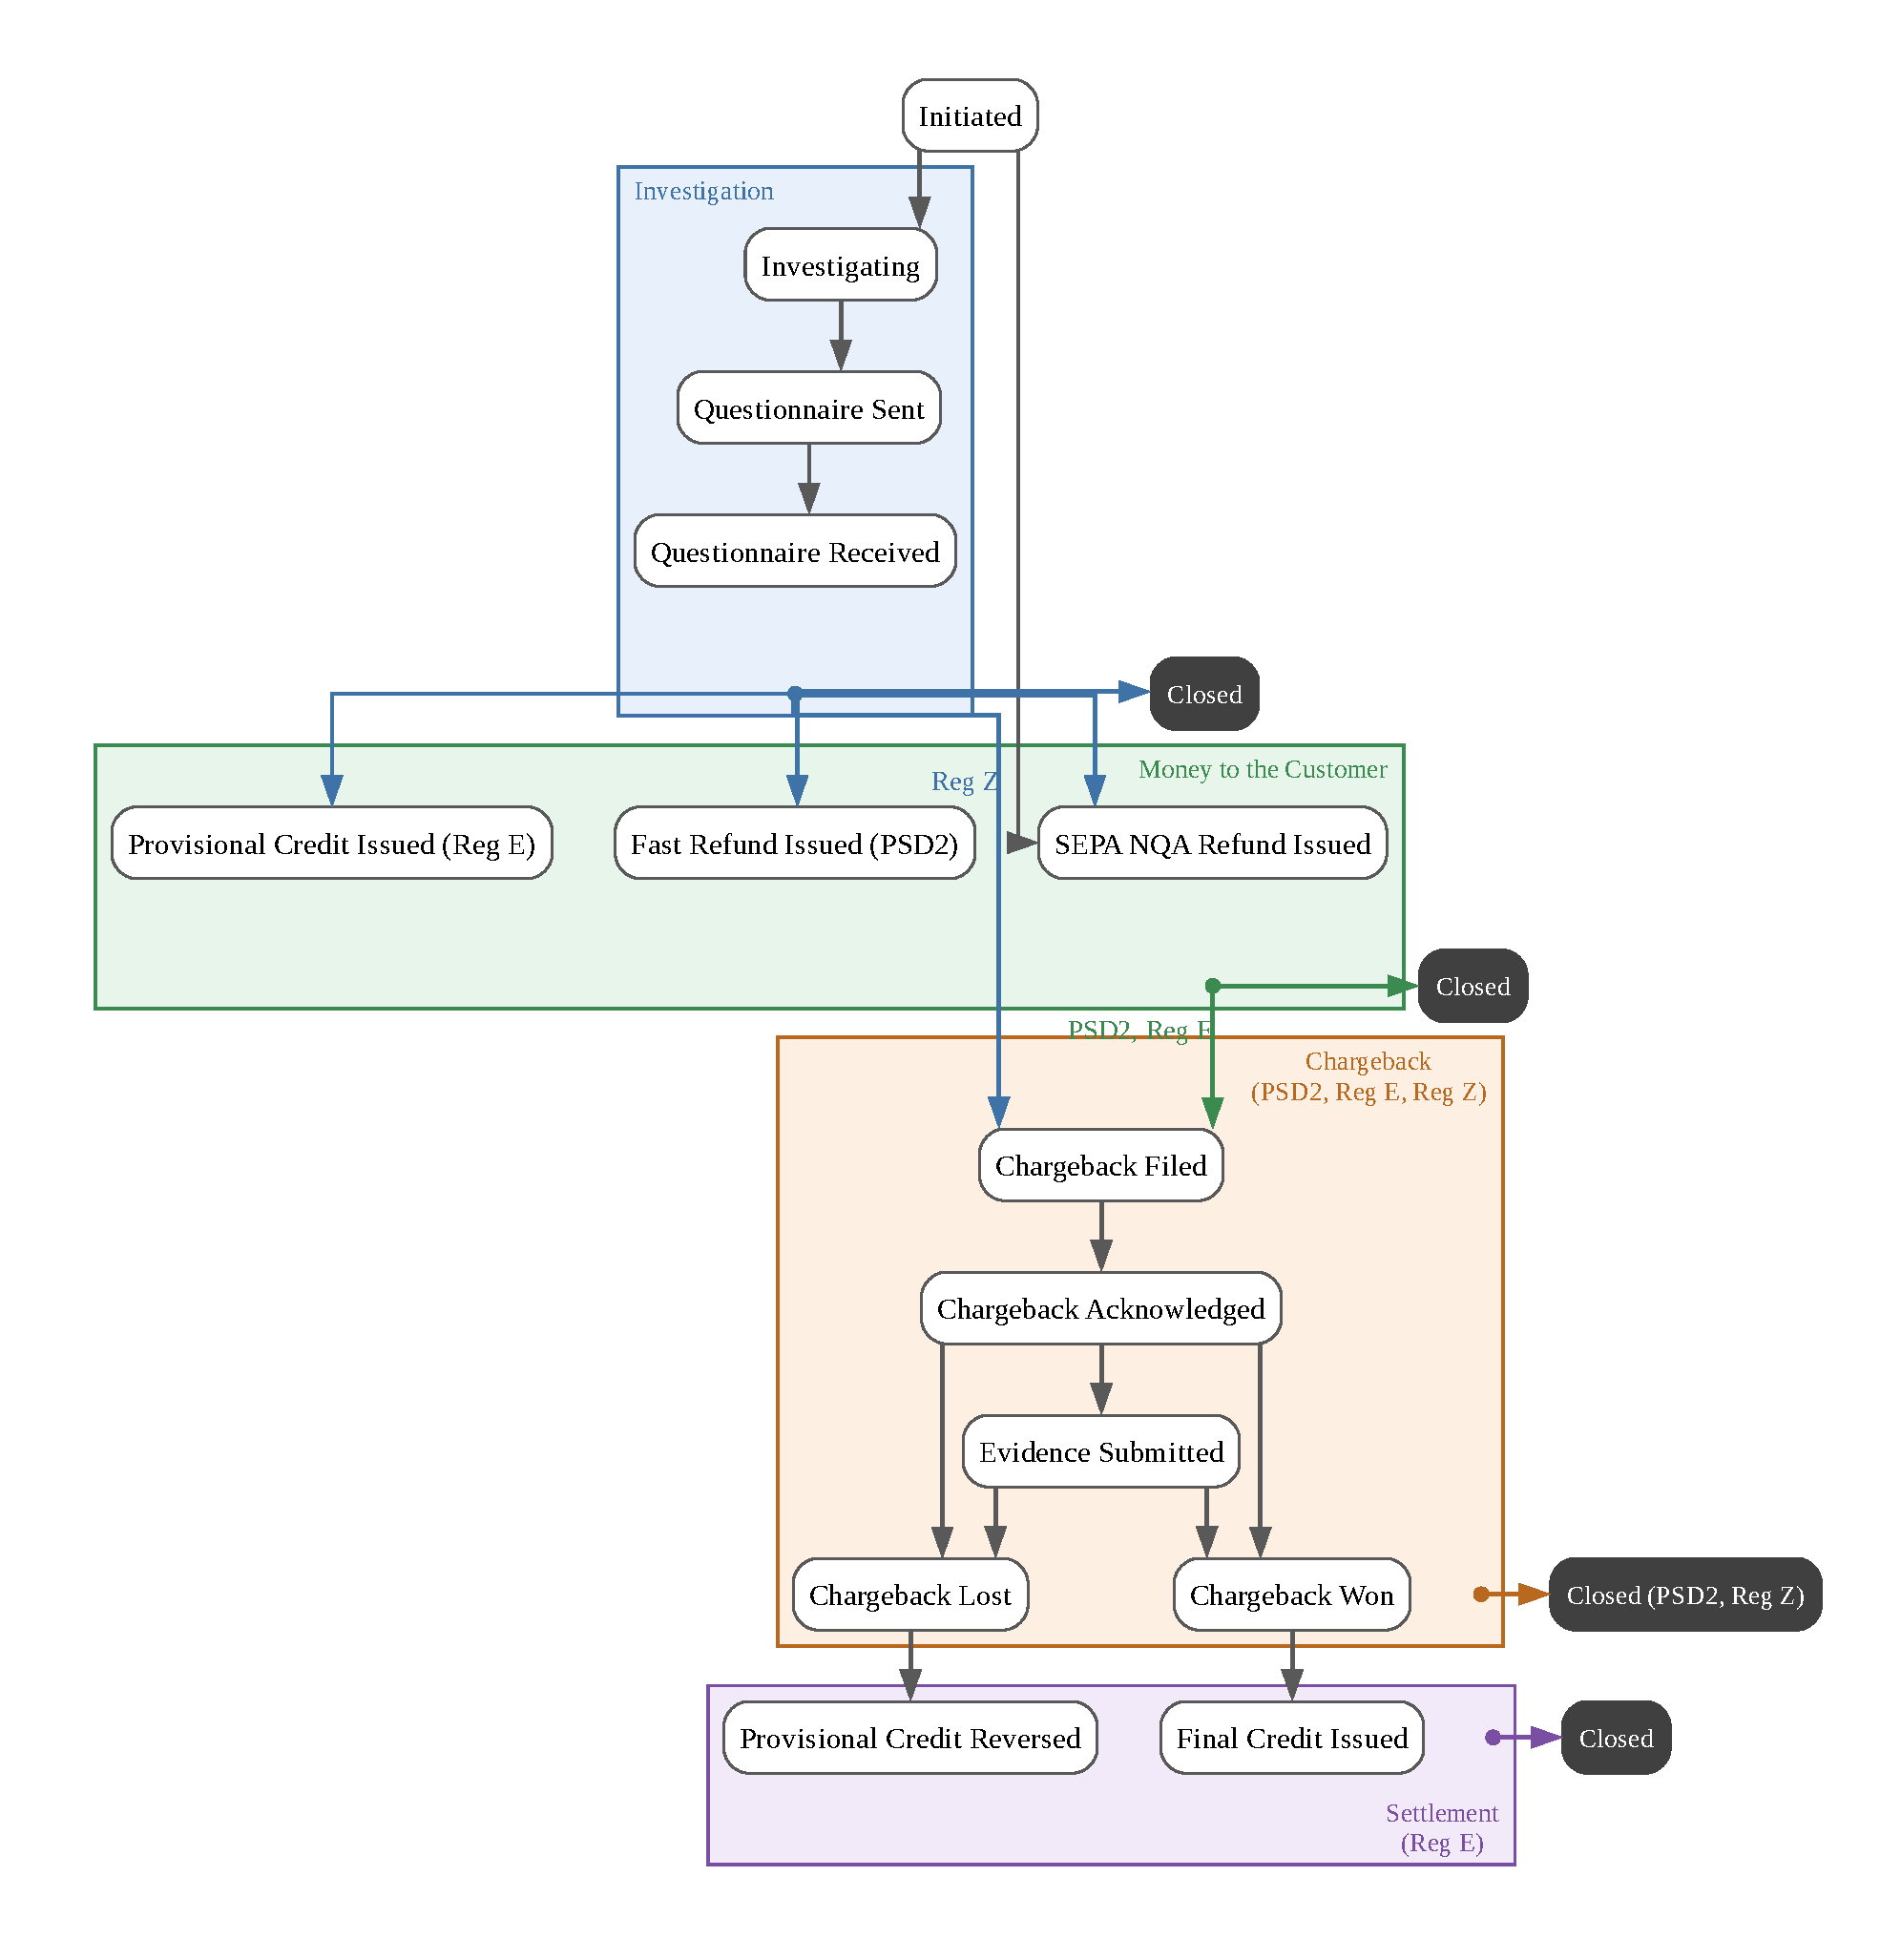
\includegraphics[width=\textwidth]{state-machine.pdf}
\caption{The dispute lifecycle under all four regimes, drawn from the transition table by a test
(\code{domain/diagram\_test.go}, \code{make thesis:figures}). Each arrow is the event that enters its target
state. Coloured boxes group the states into phases; an arrow from a dot in a phase's colour stands for the
same step taken from several of the phase's states. The dark \emph{Closed} boxes are one end state, repeated
beside each phase that can end the dispute. Names in brackets and on arrows are the regimes a state, a phase or a step is limited to (SEPA direct debit,
PSD2 card payments, Regulation~E, Regulation~Z); an unmarked arrow is open to every regime that reaches it. The appeal, from \emph{Closed} back to \emph{Investigating}
and allowed once, is not drawn.}
\label{fig:state-machine}
\end{figure}

What differs between regimes is expressed as a handful of properties of the regime's rules, never as a test
of the regime's name. The kind of money the customer receives is one: none, a no-questions-asked refund, a
fast refund or a provisional credit. Whether the regime has adjudication at all is another, and whether the
merchant may contest it a third. Whether a provisional credit exists is derived from the first. The
transition function asks these questions and nothing else. A SEPA claim can be refunded straight from
initiation, because its refund needs no investigation; a credit-card dispute under Regulation~Z files the
chargeback directly from the investigation, because there is no refund step to come first; a won chargeback
under Regulation~E cannot close until the provisional credit is made final, while under PSD2 the refund was
final all along and the dispute closes at once. The result is that the regimes reach different parts of the
same machine: six states under SEPA, eleven under PSD2, thirteen under Regulation~E and ten under
Regulation~Z. A fifth regime would be a new row of rules, its entry in the list of regimes and the branch that selects it, plus its tests, but no new code in the machine. The
regime itself is fixed when the dispute opens, from the transaction's rail and currency
(figure~\ref{fig:regimes}), and never changes afterwards, so a dispute cannot drift from one set of rules to
another halfway through.

The machine is a single pure function from a dispute and an event to the next dispute, written as one table
of cases rather than with a state-machine library. A library would have needed either one machine per
regime, which is the design that was rejected, or guard callbacks on shared transitions, which would hide
the table that the gates make readable. The function never changes the dispute it is given; it returns
the next one or refuses with an invalid-transition error, which the API reports as a \code{409} problem
(section~\ref{sec:design-failures}). The events a dispute currently offers are not listed anywhere: they are
found by asking the function about each event in turn. The workbench draws its buttons from the events the service reports, so they come from the same
computation, and a test checks the function's answers for every reachable state of every regime. An appeal is the one transition outside the table. It is allowed only from
\emph{closed}, at most once under each regime's rules, returns the dispute to the investigation, and starts
a new resolution clock (section~\ref{sec:design-clocks}).

Its tests, from the pinned set of reachable states of each regime to a gate that fails unless a named scenario
walks every accepted transition, are reported in section~\ref{sec:eval-correctness}. Figure~\ref{fig:state-machine}
is drawn from the same table by a test that compares it with a stored copy, so changing the lifecycle fails the
build until the figure is regenerated.

\section{Regulatory clocks}
\label{sec:design-clocks}

A dispute is not only a sequence of states; it is a sequence of states that must be reached by
particular dates. The dates are where the regimes differ most visibly. PSD2 requires the payer to
be refunded ``immediately, and in any event no later than by the end of the following business
day'' \cite[art.~73(1)]{psd2} and a final reply to a complaint within fifteen business days
\cite[art.~101(2)]{psd2}; for an authorised direct debit the refund or a justification is due
within ten business days of the request \cite[art.~77(2)]{psd2}. Regulation~E requires provisional
credit within ten business days and a completed investigation within forty-five days
\cite[\S~1005.11(c)]{rege}; Regulation~Z requires a written acknowledgement within thirty days and
a resolution within two billing cycles, at most ninety days \cite[\S~1026.13(c)]{regz}. Three of the
four count business days for at least one clock, which depend on the jurisdiction's holidays (Regulation~E
mixes ten business days with forty-five calendar days); the rest count calendar days. An engine that treats deadlines as documentation leaves the analyst to compute them, and
leaves the institution unable to answer the auditor's first question, namely how often it met
them.

The design carries each deadline as a \emph{clock} on the regime's rules (appendix, figure~\ref{fig:clocks}):
a kind, a count, a unit and the citation. There are three kinds, and each is defined by the states
that satisfy it rather than by the regime, in the same spirit as the gates of the state machine
(section~\ref{sec:design-state-machine}): the refund clock is met by entering any credit state,
the acknowledgement clock by sending the acknowledgement notice, the resolution clock by closing. A clock
that can no longer be met, such as the refund clock of a dispute closed without a credit, is
voided rather than breached. An appeal restarts the resolution clock and numbers the new one by the
appeal, so a dispute's history keeps every clock it ever had.

Two decisions follow from treating a due date as something the institution has told the customer.
First, the due time is computed once, when the dispute opens, and stored as a row alongside the
dispute under the same row-level security as everything else the tenant owns; a later change to a
rule or to a holiday calendar cannot silently move a deadline that was already communicated, and a
dispute opened before the feature existed has no clocks rather than an invented breach. Second,
the calendar is tenant data, not code: a tenant's settings name its time zone and public holidays,
entered at onboarding, and the due time is the last instant of the $n$th permitted day in that
zone; the unit tests in \code{domain/deadline\_test.go} fix weekends, holidays and the difference
between time zones.

Status is never stored. A clock is \emph{running}, \emph{met}, \emph{late} (satisfied after its
due time), \emph{breached} (open and past due) or \emph{void}, and the answer is a comparison of
three timestamps with the current time at the moment someone asks. Nothing therefore has to run
at midnight to notice a breach; the workbench's ``overdue only'' filter, the API's
\code{overdue} parameter and the overdue gauge all ask the same question of the same rows, and a
histogram of the slack at the moment each clock is satisfied turns compliance from a report into a
distribution.

% Distils ADR 0015.
\section{The banking core adapter}
\label{sec:design-core}

The ledger says what should move; a bank's core system moves it. Every tenant has its own, and
the proposal asked for a simulated one modelled on ISO 8583 field semantics. The simulator is the
least interesting part of the design. What matters is the port between the engine and whatever
core a tenant has: what is sent, what comes back, when the call is made, and what happens when
the answer is no, or never arrives.

An \emph{instruction} is one movement on the customer's account: the posting's reference, the
account, the amount and currency, whether it is a credit or a debit, and the dispute and original
transaction for the core's own records. A \emph{receipt} is the answer in the vocabulary a card
switch already uses: a retrieval reference number (field 37), a two-character response code
(field 39), whether the instruction was approved, and whether the core recognised the reference as
one it had already carried out (response code 94, duplicate transmission). Only postings that
touch the customer's account cross this port; suspense, recovery and loss are the bank's own books
and never leave the engine. Each tenant names its core in its settings and a router picks the
adapter by that name, so two tenants on one deployment can be two different banks; the two seed
tenants are configured differently on purpose, one refusing credits above a limit and one
answering slowly. The simulator behind the port in this build speaks the message types and fields a real
switch would, remembers what it has seen, and can be told per tenant to decline, to refuse debits
on named accounts, to be slow or to be down (\code{infrastructure/mockcore}).

The decision that shapes everything else is \emph{when} to call. The engine calls the core inside
the transition's own database transaction, with a bounded timeout, and treats the answer as part
of the transition. A decline rolls the transition back: the response is a 422 problem carrying the
core's response code, and the dispute has no new event and no new posting. Silence rolls it back
too, as a 503 the client is told to repeat with the same idempotency key. Because the transition
was never written, the repeat computes the same event sequence and therefore the same posting
reference; a core that did move the money before its answer was lost recognises the reference
and answers duplicate instead of paying twice, and the engine records that receipt as the
approval it is. The alternative, an outbox with a reconciliation job, buys the engine freedom from
the core's latency at the price of a window in which the dispute says the customer was refunded
and the core disagrees. For a system whose one job is to be right about that, the lock is the
cheaper price. Its cost is real: a slow core slows that dispute, though no other, and the test
\code{TestARetryAfterSilenceIsADuplicateNotADoublePayment} is the promise that the retry story
holds.

% Distils ADR 0014.
\section{The ledger}
\label{sec:design-ledger}

Three of the four regimes move the customer's money before anyone knows who was right. Under
Regulation~E the bank posts a provisional credit it may later take back; under PSD2 it refunds at
once and absorbs the loss unless a chargeback recovers it; under SEPA Core it refunds and the
scheme recovers the amount from the creditor's bank. The original design (appendix, wiki extract)
imagined a provisional-credit engine and a final-credit engine as separate components. Both
disappear into one small ledger once the question is put correctly: not ``what kind of credit is
this?'' but ``where is the money now?''

The ledger has four accounts from the issuer's point of view (appendix, figure~\ref{fig:ledger}): the
customer's account, a suspense account holding what the bank has advanced and not yet cleared, and
recovery and loss, which clear it. Every movement is a double-entry posting, and every posting is
caused by a transition: entering a credit state debits suspense and credits the customer; a
reversal does the opposite; a won chargeback recovers; a lost chargeback writes off, unless the
regime has provisional credit, in which case the reversal that follows takes the advance back from
the customer instead; and closing settles whatever remains, recovered or written off, by the
analyst's word or the regime's default. As with the state machine and the clocks, nothing here
tests the regime's name: the postings follow from the state entered and two properties of the
rules.

The property that matters is that suspense is zero when a dispute closes: whatever the bank
advanced was taken back, recovered or written off, and nothing is left in limbo. It is not
enforced by a check at close. It holds by construction, and the test suite proves it the way the
state machine's dead-end freedom is proved (section~\ref{sec:design-state-machine}): a test
enumerates every path from \code{INITIATED} to \code{CLOSED} under every regime, forty-three at
the time of writing, replays each through the posting rules with each settlement choice, and
asserts a zero balance and a customer who never ends up net debited
(\code{TestSuspenseBalancesOnEveryPath}). A regime or state added later that breaks the invariant
fails the build rather than a reconciliation months on.

The amount credited is the disputed amount less a liability the analyst may assign to the
customer, capped by the regime (figure~\ref{fig:regimes}). The liability
travels in the refund event's payload, as does the settlement choice on close; both are validated
against the regime before the transition is written, and a refusal is a 422 problem naming the
field, after which the dispute is exactly as it was: no event, no posting. Postings themselves are
rows under the same row-level security as the dispute, append-only at the database like the event
log, each keyed to the event that caused it and carrying a reference unique within the tenant.
That reference is the idempotency key the banking core adapter (section~\ref{sec:design-core})
uses, so an instruction repeated after a timeout cannot move money twice.

% Distils ADR 0018.
\section{Fraud scoring}
\label{sec:design-fraud}

The proposal ended with a fraud-scoring engine, marked from the outset as the first thing to
cut if time ran short. It survived in a deliberately modest form, and the form is the point.
A learned model needs labelled outcomes the project does not have and an evaluation the thesis
cannot honestly perform; and in a process where the customer has a right to know why they were
refused, a score nobody can explain is a liability rather than an asset. The engine therefore
scores with fixed, readable rules. Seven signals, each with a fixed weight and a fixed way of
earning points, each reporting a sentence that says why it scored what it did, whether or not it
fired: how many other disputes the account raised in twelve months, how many it lost at the
network, how long after the transaction the dispute came, whether the merchant's category is one
where disputes concentrate, the amount, the account's age, and the contradictions in the
questionnaire (section~\ref{sec:design-questionnaire}). The score is the sum, and two
thresholds divide it into three tiers.

Two decisions keep the score honest. It is assessed when the dispute opens, from what the engine
already knows, and assessed again when the questionnaire arrives, because that is when the
consistency signal becomes known; every assessment is kept, so the analyst sees the picture change
rather than a number that was always there. And its only teeth are a hold: a credit on a dispute
whose latest tier is high is refused until the analyst records why it should go out anyway, and
that justification is stored on the event with everything else. The score never denies a dispute,
never moves a state and never speaks to the customer. It is shown as a column of the queue and it makes a human
write a sentence before money leaves on a case the rules distrust, which is what a scoring
engine in a regulated process can responsibly do. The weights are judgement, not fitted to data;
chapter~\ref{ch:evaluation} says so and treats them as a demonstration of the mechanism rather
than a claim about fraud.

% Distils ADR 0016.
\section{The questionnaire}
\label{sec:design-questionnaire}

Two events, \code{SEND\_QUESTIONNAIRE} and \code{RECEIVE\_QUESTIONNAIRE}, have been in the state
machine from the start; until this point nothing stood behind them. The questionnaire is where the
customer's claim becomes structured data, and structure is what the investigation and the fraud
scoring (section~\ref{sec:design-fraud}) consume. Three decisions give it its shape.

First, a dispute has a \emph{reason} from the moment it opens: unauthorised transaction, goods or
services not received, duplicate charge, or an amount that differs from what was agreed. The
reason is immutable and selects the question set; the tenant systems that already open disputes
without one get the unauthorised set, which is what they were implicitly claiming. Second, the
questions are \emph{snapshotted} onto the dispute when sent. Question sets are code, and code
changes; an answer must always be readable against the exact question the customer saw, so the
sent set is stored with the dispute and a later change to the code changes nothing already sent.
Third, answers are \emph{typed facts}, not text: yes or no, a date, an amount, or free text, each
validated against the snapshot when received, with every problem reported at once and per
question, and the transition refused as a whole when any is wrong. A questionnaire answered with
``perhaps'' to a yes-or-no question is not partly received.

The immediate consumer is the analyst, who sees the answers beside the actions; the panel that
shows them is the same one that records them, since in this engine the analyst enters what the
customer said. The second consumer is the contradiction check the domain runs over the answers:
a customer who recognises the merchant, held the card, and shared it with nobody is claiming an
unauthorised payment that the answers do not support. These are sentences an analyst can act on,
and in section~\ref{sec:design-fraud} they become one of the signals a risk score is built from.

% Distils ADR 0006 and ADR 0012.
\section{The contract and its error taxonomy}
\label{sec:design-failures}

The engine is written in Go and the workbench in TypeScript, and the two share no code at runtime. What they must
share is an agreement: which requests exist, what their bodies look like, which rules a field obeys, and what each
failure means. An agreement kept in two languages by hand drifts, so the design keeps it in one place. A single
OpenAPI document is the contract, and nothing about the HTTP surface is decided anywhere else. The server's
interface is generated from it, so a route that is not in the document does not compile, and every request is
validated against the document before any handler sees it. The client's types, its request functions and the
schemas its forms validate with are generated from the same document. The generated code is committed, and the
build fails if regenerating it would change anything, so the document and both sides cannot disagree for longer
than one failed check. Only structural rules travel this way, such as a required field or the format of an
identifier; whether a transaction exists or a transition is allowed remains the server's to decide.

Failures get the same treatment, because a client that has to read error messages to decide what to do will
eventually get it wrong. Every failure the engine produces is created with a \emph{kind} and a \emph{code}. The kind
is one of nine classes, from an invalid request to an unavailable dependency, and decides the HTTP status, whether
the failure is logged and whether repeating the request can help. The code is a stable, machine-readable name such
as \code{invalid-transition}, one of 28 the contract lists. A handler never chooses a status: one table maps kind to
status for the whole service. The response is a problem document in the standard format for HTTP APIs
\cite{rfc9457}, extended with the code, whether the request is worth retrying and after how long, a reference to
the request, and, for a validation failure, one entry per field pointing at the field in the body
(figure~\ref{fig:problem}). Two codes carry what a client needs to recover: a refused transition lists the events
the dispute does allow, and a rate limit says when to come back.

\begin{figure}[htbp]
\begin{lstlisting}
HTTP/1.1 409 Conflict
Content-Type: application/problem+json

{"type": "urn:dispute-engine:error:invalid-transition",
 "title": "The request conflicts with the current state",
 "status": 409,
 "detail": "this action is not allowed in the dispute's current state",
 "instance": "/disputes/01a15551-c90d-7c55-bfe5-368b97457880/events",
 "code": "invalid-transition",
 "retryable": false,
 "requestId": "ab1de00df2f8ba20",
 "allowedEvents": ["OPEN_INVESTIGATION"]}
\end{lstlisting}
\caption{The shape of the response to an analyst who tries to win the chargeback of a PSD2 dispute that has only
just opened, as the error taxonomy renders it.}
\label{fig:problem}
\end{figure}

Everything in a problem document is written to be shown to the person who caused it. The diagnostic context that
an engineer needs, such as the regime and the state the dispute was in, is attached to the error for the logs and
the trace and never reaches the body; a test checks that it does not leak. A failure nobody classified becomes a
generic internal error whose only detail is the request reference, under which the logs and the trace hold the
cause. The list of codes is kept in two places, the contract and the Go code that emits them, and a test fails if
the two ever differ.

The workbench classifies every response once into a closed set of ten failure kinds, nine from the server's
codes and one, an unreachable server, that only a client can observe; the table from code to kind must cover every
code in the contract, which the compiler checks, and a page decides what to show from the kind, never from a
message.

% Distils ADR 0008, 0009, 0010 and 0020.
\section{Multi-tenancy with row-level security}
\label{sec:design-tenancy}

The engine serves several institutions from one deployment. They share the regulatory logic and the process;
they must never share data, and the design must not depend on every query remembering that. Three layouts were
considered: a database per tenant, a schema per tenant, and one schema in which every row names its tenant. The
first two isolate well but multiply everything an operator has to run, from migrations to dashboards, by the
number of customers. The third keeps one of everything, and is only safe if isolation is enforced somewhere a
forgotten filter cannot reach. The design takes the third and puts the enforcement in the database, with
PostgreSQL's row-level security \cite{pgrls}.

Every business table carries the tenant's identifier, and every one has the same policy: a row is visible, and
may be written, only when its tenant is the one bound to the current transaction (figure~\ref{fig:rls}). The
service binds the tenant at the start of each transaction from the authenticated caller, never from anything the
client sends, and binds it for that transaction only, so a pooled connection cannot carry one tenant's identity
into another tenant's request. When nothing is bound the setting is empty and the policy matches no rows, so
every mistake in this area fails closed; the store also refuses to open a transaction at all without a tenant.
The service runs as a database role that is subject to the policies, while the schema's owner, which runs
migrations, is not. The few things the service legitimately needs across tenants, such as the counts of disputes by state, overdue
deadlines and suspense by regime for the dashboards, the notice dispatcher's claim on the outbox, and the purges of
expired idempotency keys and draft attachments, are provided by the owner as views and functions rather than by
giving the service broader access. Idempotency keys are themselves scoped by tenant, because clients
choose them and two tenants may choose the same one.

\begin{figure}[htbp]
\begin{lstlisting}[language=SQL]
CREATE FUNCTION current_tenant_id() RETURNS uuid LANGUAGE sql STABLE AS $$
    SELECT NULLIF(current_setting('app.tenant_id', true), '')::uuid
$$;
CREATE POLICY tenant_isolation ON disputes
    USING (tenant_id = current_tenant_id())
    WITH CHECK (tenant_id = current_tenant_id());

-- at the start of every transaction (Store.WithTx), local to that transaction
SELECT set_config('app.tenant_id', $1, true);
\end{lstlisting}
\caption{The tenant policy, here on \code{disputes} (\code{migrations/0003\_tenants.sql}), and the binding the
store makes before any query. An unbound setting yields \code{NULL}, which matches no rows.}
\label{fig:rls}
\end{figure}

The tenant therefore has to come from the credential, and there are two kinds of caller with different needs.
A tenant's own systems, such as the online bank that opens disputes, run unattended and expect a credential they
can store: they present a \emph{tenant key}, a random secret shown once when it is issued and kept only as a hash,
which names its tenant and can be revoked on its own. Analysts are people, and sign in through an identity provider
\cite{oidc} in which every tenant has its own realm, so each institution's users and sign-in rules are
separate from every other's at the level of the identity system, not only by a field in a token. The tenant's short name in the address of the workbench chooses the realm before
anyone signs in. The engine verifies an analyst's token itself: the issuer of the token decides the tenant, an
issuer that no tenant owns is refused, and a tenant claim inside the token that disagrees with its issuer is
refused as a sign of a misconfigured realm. Both kinds of credential end in the same context, a tenant and a
principal, and everything below that point is shared (figure~\ref{fig:credentials}).

\begin{figure}[htbp]
\centering
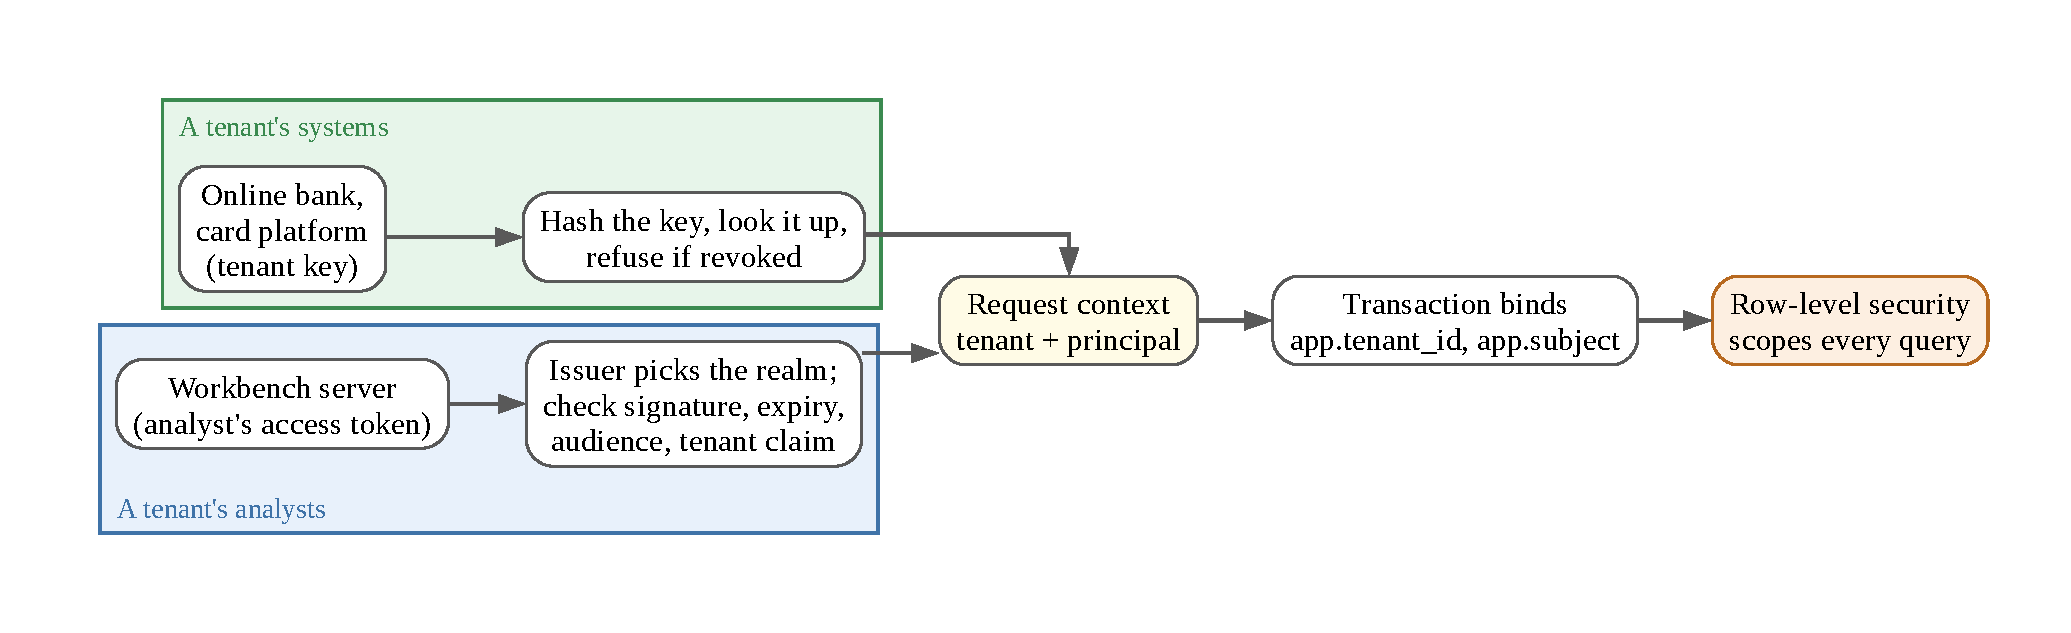
\includegraphics[width=\textwidth]{credentials.pdf}
\caption{Two kinds of credential resolving to one tenant context, which every transaction binds before its first
query so that row-level security can scope it.}
\label{fig:credentials}
\end{figure}

The browser never holds either credential; how the workbench keeps an analyst's tokens on its server is
described in section~\ref{sec:impl-sessions}. The price of the design is that
every new table needs its tenant column, its policy and its grants, and a test of the service role's grants fails before a
table without them can be released; the tenant column and the policy are a review rule rather than a test. The isolation it buys is tested against the database role
the service actually uses, as chapter~\ref{ch:evaluation} reports (section~\ref{sec:eval-isolation}).

% Distils ADR 0026.
\section{Authorization}
\label{sec:design-authorization}

Row-level security answers which tenant a row belongs to; it says nothing about who inside a
tenant may do what. Until this point the answer was everyone: any analyst or tenant key could
apply any event, including the ones that move money, and the actor written on each event was
whatever the request claimed. An issuer's own operations run on the opposite assumptions. Work
belongs to teams, seniority bounds the amounts a person may settle alone, and the person who
investigated a claim does not also pay it out. The engine therefore decides every operation that
changes a dispute or the tenant with one policy engine, over one notion of the caller.

The caller is a \emph{principal}, the same shape for both credentials of section~\ref{sec:design-tenancy}:
an analyst, named by the subject of their token and carrying whether their realm made them a
tenant administrator, or a tenant key, named by its identifier. The event actor is always this
principal and never a field of the request, so the audit trail records who acted rather than who
claimed to. That change is what makes the rest of the model meaningful, since a rule about who
opened an investigation is only as good as the record of who did.

Policies are written in Cedar \cite{cedar2024}, evaluated inside the service. Cedar was chosen over
a general-purpose policy language and over a purpose-built one for three properties the argument
depends on. It denies by default. It resolves conflicts in one fixed way: any policy that forbids
an action overrides every policy that permits it. And its semantics are specified formally, with
a reference implementation that can check a policy set against a schema before it is ever
evaluated. The engine splits its policies along that first property. \emph{Guardrails} are Cedar
in the binary that no tenant can change, mostly written as prohibitions: whoever opened the
investigation never issues its final credit, only a lead of a dispute's team may move it
elsewhere, and a tenant key never writes to a customer. The one permit gives tenant administration to the
realm role, and it is exclusive only because grants never compile to tenant resources. \emph{Grants} are data, one row per team, role and action, optionally bounded
by an amount, compiled into permissions that can reach only their own team's disputes. A grant
that cannot be expressed safely is dropped rather than escaped, so a malformed row can only take a
permission away. Because a prohibition always wins, no combination of grants can open what a
guardrail closes; that is the property that later lets tenants edit their own grants without the
engine trusting what they write.

The decision is made where the facts are committed: inside the request's transaction, after the
dispute is loaded and before the state machine runs. What the policies see is the dispute's team,
amount, rail and state, and who opened its investigation, taken from the event log rather than
from the request. A refusal names the policy that decided it, and an allowed event records the
policies that allowed it, so the log answers why a credit was permitted as well as who issued it.
The actions a dispute offers are the ones the state machine would accept and the caller may take,
so the workbench never shows a button that would be refused. Two smaller decisions close gaps the
model would otherwise leave: an idempotency key belongs to the principal that used it, so a
replayed response is never handed to someone the engine did not authorize, and the service
refuses to start if any operation in its contract has not been classified as public, internal,
open to any caller of the tenant, or decided by the engine.

% Distils ADR 0027.
\subsection{Teams, grants and a second line}
\label{sec:design-teams}

A dispute belongs to one team, chosen when it opens by the first routing rule that matches its
rail, reason and amount, and otherwise by the tenant's default team. Inside a team a person holds
one rung of a fixed ladder, junior, senior or lead, and the ladder is expressed in Cedar's own
hierarchy: a lead is a member of senior, which is a member of junior, so a grant to juniors reaches
every rung above without any role logic in code. Teams, memberships, grants and routing are rows,
and any change to them advances a version that invalidates the tenant's compiled policies on the
next request. The rows are what a tenant administrator will one day edit, and the argument of the
previous paragraphs is what makes that safe: grants compile only to permissions bounded by their
team, while everything that must always hold is a prohibition in the binary. Generated sets of
arbitrary grants confirm the three properties that matter, that no set lets an investigator pay
out their own dispute, reaches a dispute outside the caller's teams, or administers the tenant.

Team scope is enforced twice. Beside the policy decision, row-level security narrows every read to
the caller's teams, so a check forgotten in a handler still cannot show one team another's work,
and a dispute outside those teams answers as if it did not exist. The policies are restrictive
rather than permissive, a distinction with teeth: PostgreSQL combines permissive policies with
\emph{or}, so a permissive team policy beside tenant isolation would have widened what a caller
sees rather than narrowed it \cite{pgrls}. The two lines disagree in one place by design.
Reassigning a dispute to a team the lead is not in cannot pass a row policy, because an update's
new row must also be readable by the caller; that single move therefore runs as the owner,
bounded to the caller's tenant, current membership and the version they read, after the policy
engine has allowed it. What this costs per request is measured in section~\ref{sec:eval-latency}: extra round trips
rather than policy evaluation, a price of deciding inside the request's transaction on committed facts.

% Distils ADR 0017.
\section{Communications}
\label{sec:design-communications}

A dispute is a conversation with the customer as much as a sequence of states, and the regimes
say when the bank must speak: Regulation~Z wants a written acknowledgement within thirty days
\cite[\S~1026.13(c)(1)]{regz}; Regulation~E wants the customer told of a provisional credit
\cite[\S~1005.11(c)(2)(ii)]{rege}, told the date and amount of a reversal when it is debited
\cite[\S~1005.11(d)(2)]{rege}, and told the outcome with the right to see the documents relied on
\cite[\S~1005.11(d)(1)]{rege}. What the bank owes is therefore domain knowledge, and the engine
keeps it where it keeps the rest: a function from the state entered to the notices it triggers,
and a second from the regime's rules to the channels, email always and a printable letter as well
where the regime's notices must be in writing. As with the clocks and the ledger, the gate is a
property of the rules, never a regime's name.

The design question is again \emph{when}. Sending is a side effect that can fail, and a transition
must not be undone because a mail relay was down; but a notice that is owed must not be lost
because the process died between the commit and the send. The engine composes the notice inside
the transition, from facts it already holds (the account, the original transaction, the running
clocks, the ledger, the questionnaire), as structured paragraphs together with the provision the notice
satisfies, and stores it as a row in the same transaction. A letter is thereby complete the moment
it exists; the workbench lays it out on a printable page from the paragraphs, so no markup is ever
trusted. An email is an entry in an outbox, which a dispatcher drains after every commit and on a timer,
so a notice survives a crash between the commit and the send. The trade is the usual one for an
outbox: delivery is at-least-once, so a relay that accepted a message but failed to say so may
receive it twice, whereas a letter, being a row, cannot be duplicated.

Analysts also write on their own initiative, to ask for documents or to report where a case
stands, and the same machinery serves them through a small addition (ADR~0019). Their emails are
templates kept as data, each a form and a set of paragraphs in a deliberately tiny substitution
language: placeholders for the analyst's fields and for facts the engine knows, sections that appear
only when a field has a value, list-valued fields that become bullet lines. The API returns each
template with the facts already filled and the fields left as placeholders, so the browser can
preview the message live by the same substitution while the analyst types, and the server renders
the final message from the same paragraphs on send. The substitution is written twice, once for the browser and once for the server, and
no test yet makes the two equal, so preview and letter agree by construction rather than by proof; the analyst's email is a notice row like any other with its author recorded, and a machine
credential cannot compose one at all.

Two smaller consequences follow. The acknowledgement clock of section~\ref{sec:design-clocks} is
met by the acknowledgement notice, not by any state, because the acknowledgement is what the
regulation asks for. And the customer's file becomes complete and auditable from the dispute alone:
every paragraph ever sent, to which address, by which channel, and whether it went. Golden files pin the paragraphs of
every kind of notice under each regime, so a change in what a customer reads is a reviewed diff.

\chapter{Implementation}
\label{ch:implementation}

% Budget and sources: docs/thesis/outline.md. Every claim about behaviour points at a test, a figure or a number in data/.

\section{The service and its persistence}
\label{sec:impl-service}

The engine is one Go program using the standard library's HTTP server and router and nothing above them, so
every behaviour that wraps a request, from panic recovery to authentication and the rate limit, is a small piece
of code in the repository rather than a framework's convention. The code follows the layers of the
design (figure~\ref{fig:layers}). The \code{dispute} context has a pure domain layer with no input or output at
all, which is why chapter~\ref{ch:design} can describe the state machine, the clocks and the ledger as functions;
an application layer of use cases that orchestrate it; infrastructure adapters for the database, the mail relay
and the simulated core; and HTTP ports that implement the generated interface.

\begin{figure}[htbp]
\centering
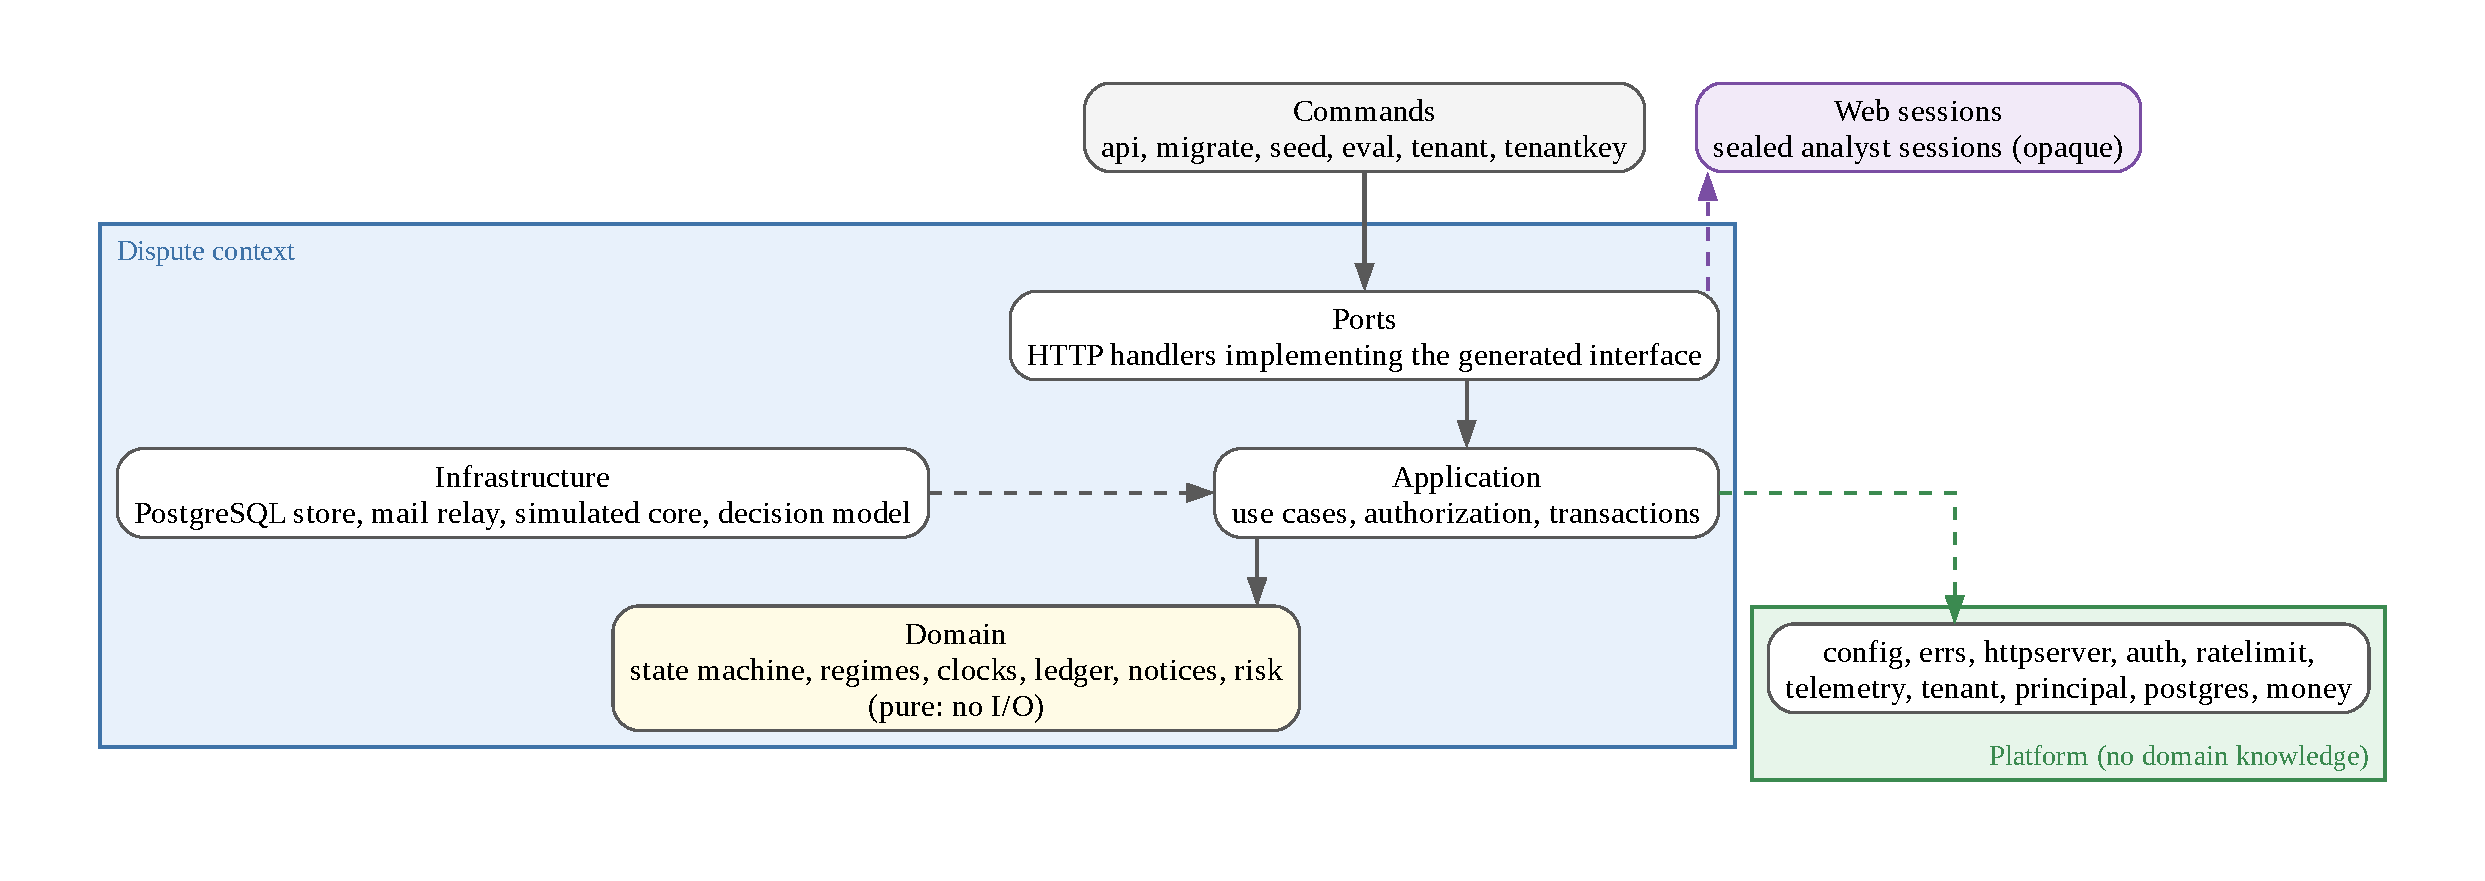
\includegraphics[width=\textwidth]{layers.pdf}
\caption{The layers of the service. Solid arrows are calls; the infrastructure implements interfaces the
application declares, so the application never imports it; the domain does no input or output. The web-session
package stores the workbench's sealed sessions (section~\ref{sec:impl-sessions}).}
\label{fig:layers}
\end{figure}

PostgreSQL is the only stateful dependency. Every mechanism that is often given its own system lives in the
database instead, inside the same transaction and the same trace as the work it serves: the idempotency store,
the per-tenant rate-limit counters, the analysts' sessions, the outbox of emails, and the one-at-a-time lock for
background sweeps; the evaluation found its queries well under a millisecond at the 95th percentile
(section~\ref{sec:eval-latency}). A dispute is stored as a row holding its current state and a version, beside an
append-only log of every transition. A transition reads the row, runs the state machine in memory and writes back
only if the version is still the one it read; a concurrent writer that got there first makes the write affect no
row, and the caller receives a conflict instead of waiting on a lock \cite{kleppmann2017}.

The 83 queries are written in SQL and compiled into typed Go functions, so a column renamed in a migration breaks
the build rather than a request. The 24 migrations run forward only, applied by a separate command under the
schema owner's role; the service checks the schema version when it starts and refuses to serve behind it. The
service itself connects as a login that can read and insert where it must and cannot alter the schema or rewrite
the event log; a test checks the login's privileges, and the event log's triggers refuse a rewrite even from the
owner (section~\ref{sec:eval-log}).

The schema behind this is drawn in figure~\ref{fig:erd}, generated from the migrated database rather than drawn by
hand, so it cannot describe a schema that no longer exists. Every table carries its tenant, and the dispute's
satellites (events, clocks, postings, questionnaires, notices and risk assessments) hang off the dispute row by its
identifier and the event's sequence number, which is how a posting or a notice can always be traced to the
transition that caused it.

\begin{sidewaysfigure}
\centering
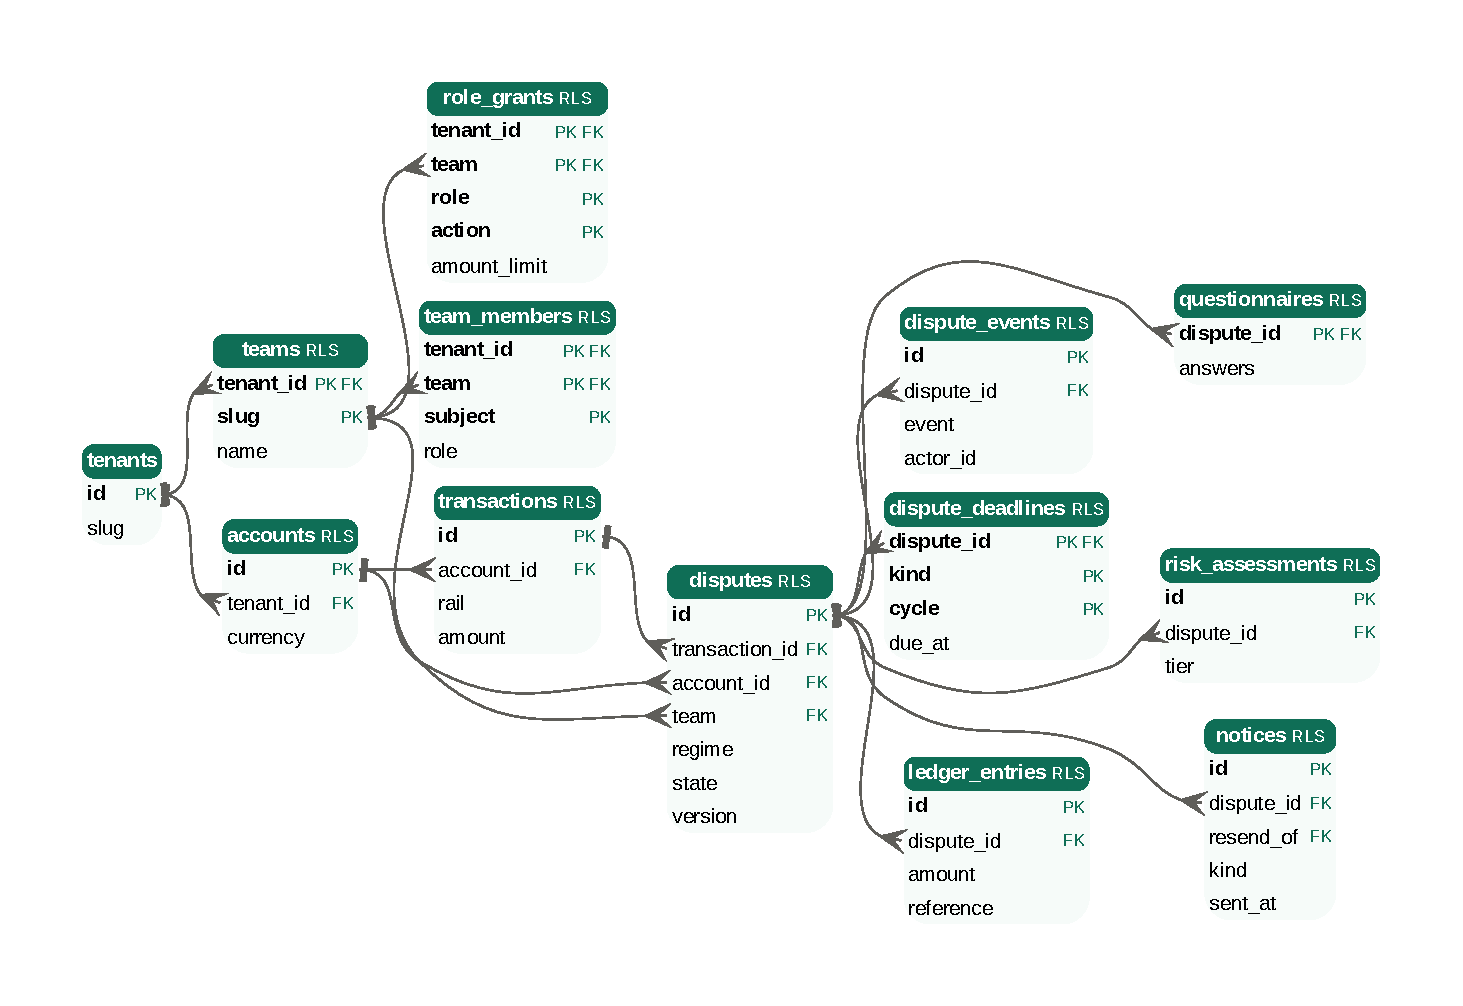
\includegraphics[width=\textheight,height=0.8\textwidth,keepaspectratio]{erd.pdf}
\caption{The core tables of the schema and their foreign keys, generated from the migrated database by
\code{scripts/erd}; 13 of the 23 tables are shown. Primary keys are bold. Every table drawn also references
\code{tenants} through its \code{tenant\_id}; only the first links are drawn. RLS marks a table under the
row-level security policy of figure~\ref{fig:rls}.}
\label{fig:erd}
\end{sidewaysfigure}

\section{The state machine and the regime rules in code}
\label{sec:impl-state-machine}

The regimes of table~\ref{tab:regimes} are one Go map from the regime to a value of type \code{Rules}
(figure~\ref{fig:rules}). Each row carries the properties the transition function is allowed to ask about, the
regime's clocks with their legal basis as a string the workbench displays, the customer's liability cap in minor
units, and two settings the ledger and the notices read: how a dispute closed without adjudication settles its
suspense, and whether the regime requires notices in writing. Money is never a floating-point number anywhere in the
engine; amounts are decimals in the domain and integers of minor units at the boundaries.

\begin{figure}[htbp]
\begin{lstlisting}
// domain/regime.go
type Rules struct {
	Regime             Regime
	Refund             RefundPath   // none, provisional, fast or NQA
	Clocks             []Clock
	HasAdjudication    bool
	MerchantMayContest bool
	LiabilityCapMinor  int64
	MaxAppeals         int
	CloseSettlement    SuspenseSettlement
	WrittenNotices     bool
	// ...
}

RegimeEUPSD2Card: {
	Refund: RefundFast,
	Clocks: []Clock{
		{Kind: DeadlineRefund, Count: 1, Unit: BusinessDays,
		 Basis: "PSD2 art. 73(1): refund by the end of the following ..."},
		{Kind: DeadlineResolution, Count: 15, Unit: BusinessDays,
		 Basis: "PSD2 art. 101(2): final reply to a complaint within ..."},
	},
	HasAdjudication:    true,
	MerchantMayContest: true,
	LiabilityCapMinor:  50_00, // EUR 50.00 in minor units
},
\end{lstlisting}
\caption{The type a regime contributes to the engine and its row for PSD2 card payments (abridged). The other three
rows have the same shape; the full set of clocks is table~\ref{tab:clocks}.}
\label{fig:rules}
\end{figure}

The transition function is \code{Dispute.Apply}, a method on a small value holding the regime, the state and the
number of appeals used. It returns a new value rather than changing the old one, so a caller that discards the
result has changed nothing, and it performs no input or output. Inside it, one \code{switch} on the current state
and one on the event decide the destination, and every condition in it is a property of the rules
(figure~\ref{fig:apply}). The one exception, the appeal, is handled before the table, because it alone needs the
counter of appeals already used.

\begin{figure}[htbp]
\begin{lstlisting}
// domain/state.go: next gates on Rules properties, never on the Regime
case StateChargebackWon:
	switch e {
	case EventIssueFinalCredit:
		// Regulation E: the provisional credit must be made final first
		if r.HasProvisionalCredit() {
			return StateFinalCreditIssued, true
		}
	case EventClose:
		// PSD2 and Regulation Z: nothing is left to settle
		if !r.HasProvisionalCredit() {
			return StateClosed, true
		}
	}
\end{lstlisting}
\caption{One case of the transition table: a won chargeback. The same two lines serve all four regimes because they
ask whether a provisional credit exists, not which regime the dispute is under.}
\label{fig:apply}
\end{figure}

What the workbench may offer is not a second table. \code{Dispute.Allowed} tries every event against
\code{Apply} and returns those it accepts, and the API returns that list with every dispute, so the buttons on the
dispute page and the \code{allowedEvents} of a refusal (figure~\ref{fig:problem}) are produced by the same function
that enforces the rule. The lifecycle diagram of figure~\ref{fig:state-machine} is produced the same way: a test
walks \code{Apply} for every regime, state and event and writes the graph, so the figure in this document is
regenerated from the code rather than maintained beside it.

\section{One transition, end to end}
\label{sec:impl-transition}

An analyst pressing a button on the dispute page becomes one call to the use case \code{ApplyEvent}, and every
side effect a transition has happens inside that call and inside one database transaction. The order of the steps
is the design of chapter~\ref{ch:design} made concrete (figure~\ref{fig:apply-event}).

\begin{figure}[htbp]
\begin{lstlisting}
// application/service.go (abridged; any error rolls the whole call back)
return s.idempotent(ctx, "dispute.apply_event", in.Idempotency,
	func(tx Tx) (DisputeView, error) {
		rec, _ := tx.GetDispute(ctx, in.DisputeID) // row-level security
		f, _ := facts(ctx, tx, rec)                // committed facts
		dec, _ := s.authorize(ctx, tx, action, &f) // Cedar policies
		next, _ := rec.Lifecycle().Apply(in.Event) // the state machine
		s.holdCheck(ctx, tx, rec, in.Payload)      // the fraud hold
		tx.UpdateDisputeState(ctx, rec.ID, rec.Version, next.State, ...)
		tx.AppendEvent(ctx, rec.ID, EventRecord{Seq: int(rec.Version) + 1, ...})
		s.questionnaire(ctx, tx, rec, in.Event, payload, now) // send or record
		s.settleDeadlines(ctx, tx, rec, next, now)       // meet or void clocks
		s.post(ctx, tx, rec, next, ev.Seq, payload, now) // ledger and core
		s.notify(ctx, tx, rec, next.State, ev.Seq, now)  // letters and emails
		// ... reassess the score after a questionnaire, record metrics
		return s.viewWith(ctx, tx, rec, &f)
	})
\end{lstlisting}
\caption{The use case behind every button on the dispute page. Because each step runs inside the same
transaction, a refusal at any step, from the policy engine to the banking core, leaves no trace of the attempt.}
\label{fig:apply-event}
\end{figure}

The transaction itself is opened by the store, which first binds the caller's tenant to it
(figure~\ref{fig:rls}) and, for an analyst, the caller's identity, which the team policies of
section~\ref{sec:design-authorization} read. The dispute row is then read under those policies, so a dispute of
another tenant or another team is simply not found. The facts the policy engine decides on are assembled from the
row and from the event log, which is where the identity of the investigator lives, and the decision is taken
before the state machine is even asked. The two refusals therefore stay distinct: \code{403} means the caller may not
do this, \code{409} that nobody may do it from this state.

The write is guarded by the version that was read. \code{UpdateDisputeState} changes the row only where its version
still equals the one the use case started from, and a write that matches no row is reported as a conflict that the
client may retry after reloading; nothing waits on a lock, and two analysts pressing different buttons at the same
moment cannot both succeed. The event appended next takes its sequence number from the same version, so the log has
no gaps and a uniqueness constraint on the pair of dispute and sequence makes a second writer fail even if the
version check were removed. The event records the actor taken from the authenticated principal and the
identifiers of the policies that allowed it.

The wrapper \code{idempotent} makes the whole call repeatable. A client sends a key with every write; the wrapper
stores the hash of the request body and the response under that key, scoped to the caller, in the same
transaction as the work. A repeat with the same key and the same body returns the stored response and does nothing
else; the same key with a different body is refused, because it is a bug in the client rather than a retry. Only
after a successful commit does the use case wake the email dispatcher, so an email is never sent for a transition
that was rolled back.

\section{Clocks, postings and the banking core}
\label{sec:impl-money}

A due date is computed by walking the tenant's calendar forward one day at a time (figure~\ref{fig:due}). The
calendar holds a time zone and a set of holiday dates read from the tenant's settings; a business day is a weekday
that is not one of them. The deadline is the last instant of the final counted day in the tenant's zone, so a PSD2
refund owed ``by the end of the following business day'' is due at midnight in Budapest for the seeded tenants, not in the server's zone.
The unit tests pin weekends, a Hungarian national holiday and the tenant's zone rather than the server's.

\begin{figure}[htbp]
\begin{lstlisting}
// domain/deadline.go
func (c Calendar) Due(start time.Time, clock Clock) time.Time {
	loc := c.loc()
	day := start.In(loc)
	day = time.Date(day.Year(), day.Month(), day.Day(), 0, 0, 0, 0, loc)
	for n := 0; n < clock.Count; {
		day = day.AddDate(0, 0, 1)
		if clock.Unit == CalendarDays || c.IsBusinessDay(day) {
			n++
		}
	}
	// the end of the last counted day
	return day.AddDate(0, 0, 1).Add(-time.Nanosecond)
}
\end{lstlisting}
\caption{The due date of a clock in the tenant's calendar. The count starts on the day after the dispute opens.}
\label{fig:due}
\end{figure}

The ledger of table~\ref{tab:ledger} is a pure function too: given the rules, the state entered, the disputed amount,
the liability and the suspense balance already outstanding, \code{domain.Postings} returns the movements to write.
The use case turns each movement into a row whose reference is built from the dispute, the event's sequence number
and the kind of posting, for example \code{dispute:<id>:7:credit}. The reference is therefore the same however many
times the request is repeated, and it is what the banking core is given as its idempotency key.

Only the movements that touch the customer's account are sent to the core; suspense, recovery and loss are the
bank's own books. The port, \code{BankingCore}, has a single method that takes the tenant's core configuration and
an instruction and returns a receipt, and it returns an error only when no answer came, so a decline and a silence
can never be confused. The simulated core translates each instruction into the ISO~8583 fields a real switch would
see: a financial request message, a processing code that says whether the account is credited or debited, the
amount in minor units, the numeric currency, and a retrieval reference number derived from the posting's reference
(figure~\ref{fig:iso}). It remembers every reference it approved and answers a second request for one with response
code 94, duplicate transmission, and the original authorisation. Its behaviour is set per tenant: a limit above
which credits are declined with code 61, accounts that refuse debits with code 51, an artificial delay, or a
complete outage. The trace of every transition shows the message, so the exchange can be inspected in the running
system (figure~\ref{fig:trace}).

\begin{figure}[htbp]
\begin{lstlisting}
{"mti": "0200", "de3": "200000", "de4": "000000004200", "de7": "1107142231",
 "de11": "000017", "de37": "3F9A1C07B2E4", "de49": "978", "de102": "8f1c..."}
{"mti": "0210", ..., "de37": "3F9A1C07B2E4", "de38": "3F9A1C", "de39": "00"}
\end{lstlisting}
\caption{The shape of the request and response the simulated core logs for a fast refund of EUR 42.00 (illustrative
values, abridged): field 3 says
the account is credited, field 37 is derived from the posting's reference, and field 39 is the response code.}
\label{fig:iso}
\end{figure}

The call is bounded by a timeout. A decline becomes a \code{422} problem whose detail carries the core's response
text and code; a timeout or an outage becomes a \code{503} the client retries with the same idempotency key. In both
cases the database transaction is rolled back, so the dispute is still in its old state and has no posting that
the core did not confirm.

\section{Notices and the email outbox}
\label{sec:impl-notices}

The notices of section~\ref{sec:design-communications} are composed during the transition from facts the
transaction already holds: the customer, the amounts, the clocks and the provision that requires the notice. A notice
is stored as structured paragraphs rather than as rendered text, so the same row produces the email and the
printable letter, and golden files pin the paragraphs for every regime and state that owes one.

The emails leave through an outbox table drained by a dispatcher that is woken after every commit and also runs on
a timer. Claiming a batch is one statement (figure~\ref{fig:outbox}): it picks the emails that are due, skips any
row another replica has already locked, and pushes each one's next attempt back exponentially, from thirty seconds
to at most an hour, before the send is even tried. A process that dies mid-send therefore leaves the email to be
claimed again later rather than lost, and a relay that is down receives fewer and fewer attempts rather than a flood.
The dispatcher has no tenant of its own, so the claim is a function owned by the schema's owner, granted to the
service and nothing else.

\begin{figure}[htbp]
\begin{lstlisting}[language=SQL]
UPDATE notices n
SET attempts = n.attempts + 1,
    next_attempt_at = now()
        + make_interval(secs => least(3600, 30 * power(2, n.attempts)))
WHERE n.id IN (
    SELECT id FROM notices
    WHERE sent_at IS NULL AND channel = 'EMAIL' AND next_attempt_at <= now()
    ORDER BY next_attempt_at
    LIMIT batch
    FOR UPDATE SKIP LOCKED)
RETURNING n.*;
\end{lstlisting}
\caption{Claiming a batch of emails from the outbox (\code{claim\_notices}, \code{migrations/0020\_notice\_trace.sql}).
Each row stores the trace context of the transition that owed it, so its delivery joins that transition's trace.}
\label{fig:outbox}
\end{figure}

\section{Fraud signals and the hold}
\label{sec:impl-fraud}

\code{domain.Assess} is a function from a set of facts about the dispute, its account and its questionnaire to an
assessment: a list of signals, each with its maximum weight, the points it contributed and a sentence saying why,
and the tier the total falls into, medium from 20 points and high from 45. The sentences are what the dispute page
shows beside the score (figure~\ref{fig:dispute}), so an analyst never sees a number without its reasons. The
facts are read inside the transaction that opens the dispute and again in the one that records the questionnaire,
and each assessment is stored as a new row, never updated.

The hold is a single check in the refund step of figure~\ref{fig:apply-event}: if the latest assessment is high, a
refund or credit is refused with a \code{422} problem that names the missing field unless the request carries a non-empty justification, which is then
stored in the event's payload and shown in the log. The score has no other effect on the code path.

\section{Policies in code}
\label{sec:impl-policies}

The guardrails of section~\ref{sec:design-authorization} are a Cedar file compiled into the binary
(figure~\ref{fig:guardrails}). Each policy carries an identifier, and the identifiers of the policies that decided a
request are what the event log and a refusal report. The policy set is validated against a Cedar schema in
continuous integration, so a policy that names an attribute the engine never supplies fails the build rather than
silently denying.

\begin{figure}[htbp]
\begin{lstlisting}
// Separation of duties: the investigator never issues the final credit.
@id("sod-final-credit")
forbid (principal is Analyst, action == Action::"ISSUE_FINAL_CREDIT",
        resource is Dispute)
when { resource.investigationOpenedBy == principal.id };

// Only a lead of the dispute's team may move it to another team.
@id("reassign-leads-only")
forbid (principal, action == Action::"reassign", resource is Dispute)
unless { principal is Analyst && principal.leadOf.contains(resource.team) };

// compiled from one grant row: seniors of "cards" refund up to 5000
@id("grant:cards/senior/ISSUE_REFUND")
permit (principal in TeamRole::"cards/senior",
        action == Action::"ISSUE_REFUND",
        resource in Team::"cards")
when { resource.amount.lessThanOrEqual(decimal("5000.0000")) };
\end{lstlisting}
\caption{Two of the guardrails (\code{authz/policy/guardrails.cedar}) and a permit compiled from a grant row by
\code{authz.Compile}.}
\label{fig:guardrails}
\end{figure}

Grants are compiled per tenant into permits like the last one in the figure, and the compiled set is cached per tenant
under the version of its grants, so a change to a grant takes effect on the next request. The compiler accepts only the roles the engine knows and team names and actions made of a
small set of safe characters, and it skips any row outside them rather than escaping it, so a grant can never
inject policy text. The property tests of section~\ref{sec:design-authorization} generate grant sets, compile them
and check the three properties through the same engine the service uses.

\section{One contract, two generated sides}
\label{sec:impl-contract}

One command regenerates everything derived on the server from the contract of section~\ref{sec:design-failures}:
the typed queries from the SQL, and the server interface, the request and response types and the validator from
the OpenAPI document. A second command regenerates and compares the result with what is committed, failing with
the list of files that differ, and continuous integration runs the same regeneration and comparison. On the
client, a script reads the same document and writes two files (figure~\ref{fig:contract}): the TypeScript types
and request functions, and a validation schema for every component schema in the document.

The two client files come from different libraries and could disagree, so each generated schema is followed by an
assertion that the type it validates is exactly the type generated for the same component
(figure~\ref{fig:schema-pair}); a schema that drifted from its type is a compile error, not a surprise in a form.
The workbench validates in one place only: a module that accepts any schema in the common Standard Schema
interface, adapts the generated ones behind it, and returns either the value or one error per field. Forms use it
before they submit, and every server function uses it on its input before it calls the engine.

\begin{figure}[htbp]
\centering
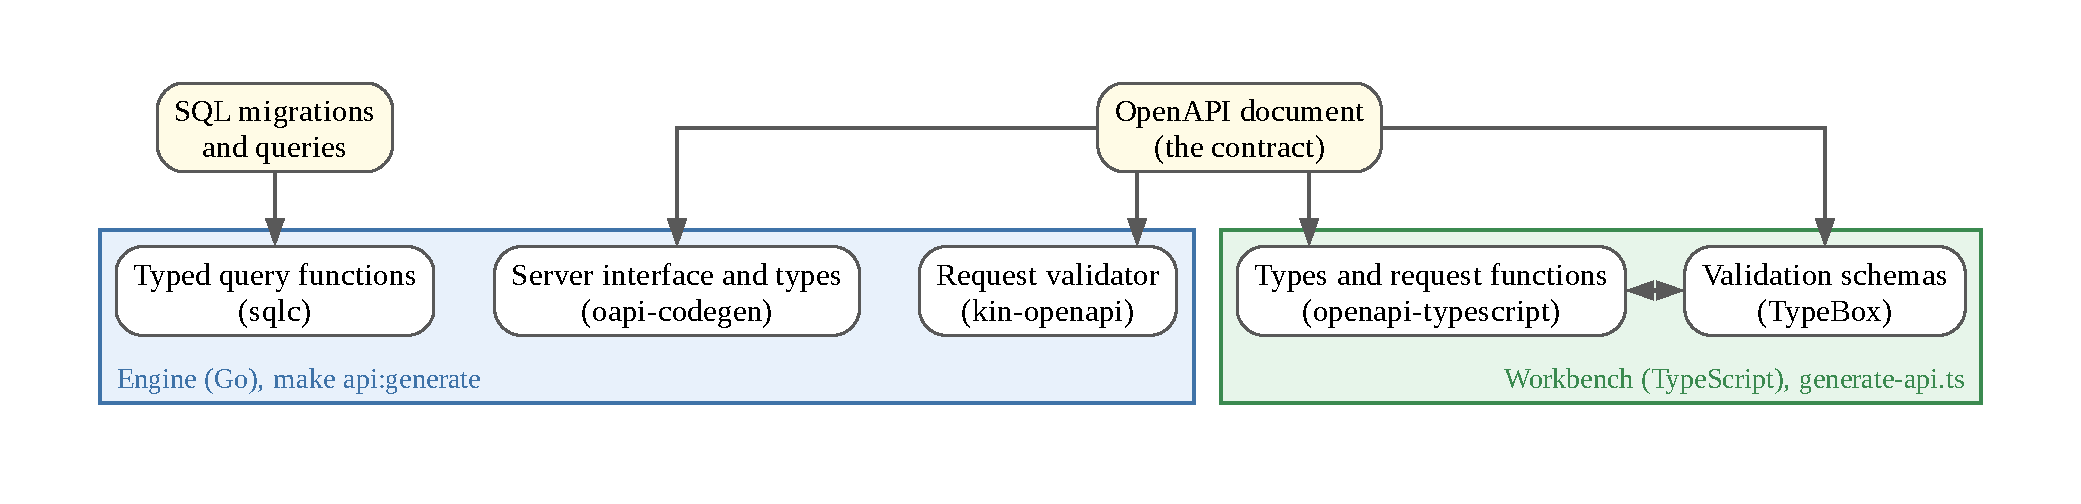
\includegraphics[width=\textwidth]{contract.pdf}
\caption{What is generated from the contract and the SQL on each side. The dashed arrow is the compile-time check
that each validation schema's type equals the generated type of the same component (figure~\ref{fig:schema-pair});
continuous integration regenerates everything and fails on any difference from what is committed.}
\label{fig:contract}
\end{figure}

\begin{figure}[htbp]
\begin{lstlisting}
# docs/api/openapi.yaml
CreateDisputeRequest:
  type: object
  required: [transactionId]
  properties:
    transactionId: { type: string, format: uuid }
    reason: { $ref: "#/components/schemas/DisputeReason" }
    suggestion: { $ref: "#/components/schemas/AcceptedSuggestion" }

// frontend/src/api/schemas.gen.ts (generated)
export const CreateDisputeRequest = Type.Object({
  transactionId: Type.String({ format: 'uuid' }),
  reason: Type.Optional(DisputeReason),
  suggestion: Type.Optional(AcceptedSuggestion),
})
export type CreateDisputeRequest = Static<typeof CreateDisputeRequest>
const _CreateDisputeRequest: Same<CreateDisputeRequest,
  components['schemas']['CreateDisputeRequest']> = true
\end{lstlisting}
\caption{One component of the contract (descriptions omitted) and the validation schema generated from it. The
last line compiles only if the schema's type equals the type generated for the same component.}
\label{fig:schema-pair}
\end{figure}

\section{Sessions and sign-in}
\label{sec:impl-sessions}

An analyst signs in through an address ending in the tenant's short name (figure~\ref{fig:signin}), which starts
the authorization-code flow with proof-key protection against that tenant's realm. The callback validates the identity token, creates a new
session identifier and gives the browser a cookie carrying only that identifier, which scripts cannot read and
which the browser does not attach to requests other sites make in the background.

The workbench has no database connection of its own. It seals the session's contents, the analyst's identity and
tokens, with authenticated encryption under a key only the workbench server holds, and stores the sealed result
through internal endpoints of the engine that accept a service key rather than a tenant's credential. The engine
keeps the ciphertext and an expiry, enforces the expiry on every read and sweeps expired rows, but cannot read
what it stores; neither can anyone holding a copy of the database.

\begin{figure}[htbp]
\centering
\resizebox{\textwidth}{!}{% Figure: analyst sign-in sequence (docs/authentication.md, ADR 0011, 0020). Drawn in TikZ so Overleaf compiles it unchanged.
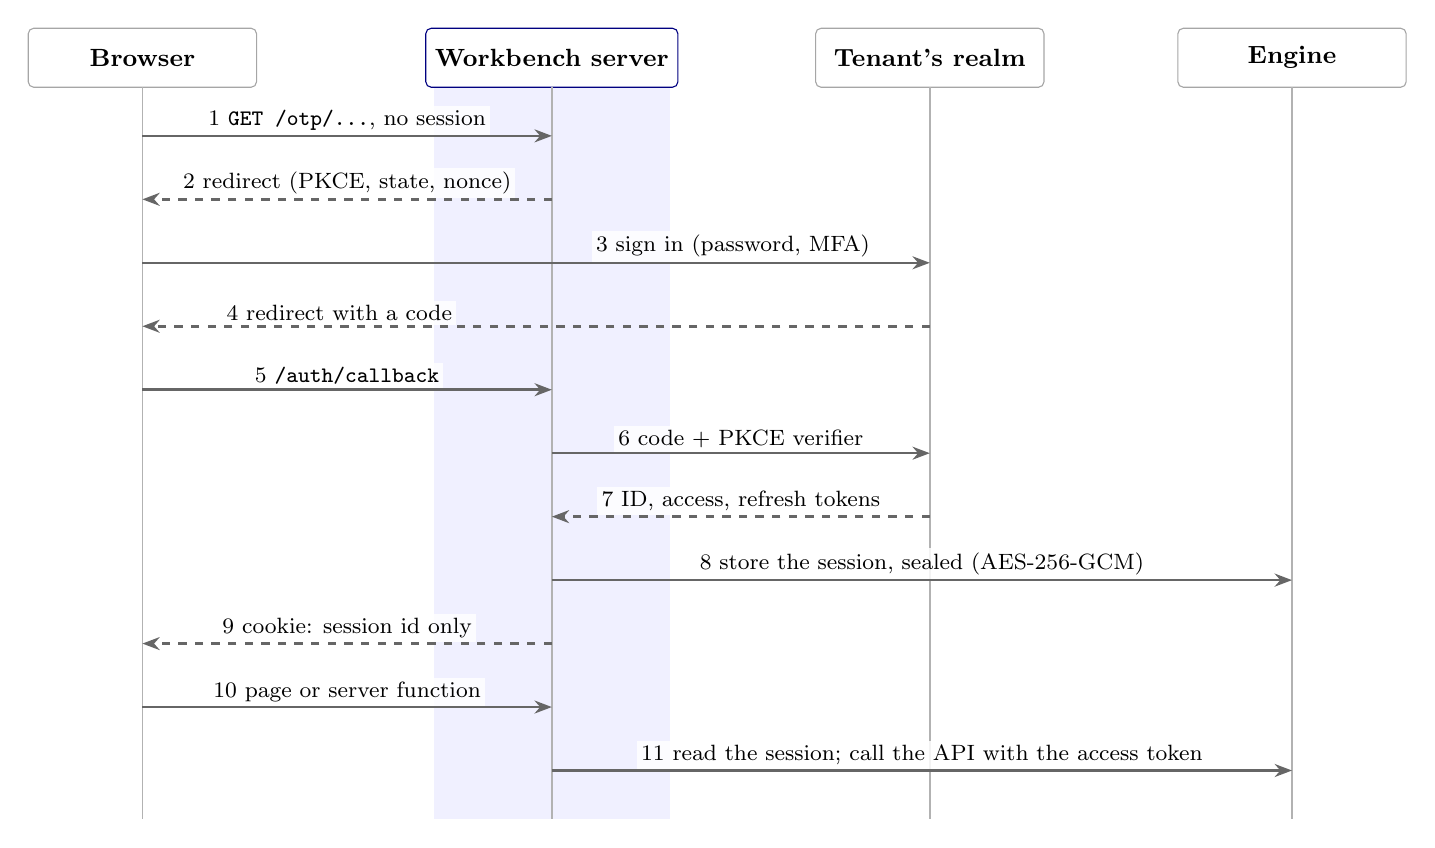
\begin{tikzpicture}[x=1cm,y=-0.62cm,font=\small,
  actor/.style={draw=gray!70,rounded corners=2pt,fill=white,minimum width=2.9cm,minimum height=0.75cm,align=center,font=\small\bfseries},
  msg/.style={-{Stealth[length=2.2mm]},line width=0.9pt,draw=gray!80!black},
  ret/.style={msg,dashed},
  lbl/.style={above,font=\footnotesize,align=center,inner sep=1.5pt,fill=white,fill opacity=0.85,text opacity=1}]
  \def\B{0}\def\W{5.2}\def\R{10.0}\def\E{14.6}
  \fill[blue!6] (\W-1.5,0.6) rectangle (\W+1.5,15.6);
  \node[actor] at (\B,0) {Browser};
  \node[actor,draw=blue!50!black] at (\W,0) {Workbench server};
  \node[actor] at (\R,0) {Tenant's realm};
  \node[actor] at (\E,0) {Engine};
  \foreach \x in {\B,\W,\R,\E} \draw[gray!60,line width=0.6pt] (\x,0.6) -- (\x,15.6);
  \draw[msg] (\B,1.6) -- node[lbl]{1 \texttt{GET /otp/...}, no session} (\W,1.6);
  \draw[ret] (\W,2.9) -- node[lbl]{2 redirect (PKCE, state, nonce)} (\B,2.9);
  \draw[msg] (\B,4.2) -- node[lbl,pos=0.75]{3 sign in (password, MFA)} (\R,4.2);
  \draw[ret] (\R,5.5) -- node[lbl,pos=0.75]{4 redirect with a code} (\B,5.5);
  \draw[msg] (\B,6.8) -- node[lbl]{5 \texttt{/auth/callback}} (\W,6.8);
  \draw[msg] (\W,8.1) -- node[lbl]{6 code + PKCE verifier} (\R,8.1);
  \draw[ret] (\R,9.4) -- node[lbl]{7 ID, access, refresh tokens} (\W,9.4);
  \draw[msg] (\W,10.7) -- node[lbl,pos=0.5]{8 store the session, sealed (AES-256-GCM)} (\E,10.7);
  \draw[ret] (\W,12.0) -- node[lbl]{9 cookie: session id only} (\B,12.0);
  \draw[msg] (\B,13.3) -- node[lbl]{10 page or server function} (\W,13.3);
  \draw[msg] (\W,14.6) -- node[lbl,pos=0.5]{11 read the session; call the API with the access token} (\E,14.6);
\end{tikzpicture}
}
\caption{An analyst of the tenant \code{otp} signing in. The tokens stay on the workbench server (shaded); the
engine stores the session sealed and cannot read it, and the browser holds only the session's identifier.}
\label{fig:signin}
\end{figure}

Tokens are refreshed only on the server. A session ends in
one of four ways: the analyst signs out, which also ends the identity provider's session; thirty minutes pass
without activity; the identity provider's ten-hour maximum session ends; or the identity provider tells the
workbench directly, by back-channel logout, that the analyst was signed out elsewhere or disabled, which ends the
workbench sessions tied to that identity-provider session.

\section{The analyst workbench}
\label{sec:impl-workbench}

The decision that shapes the workbench is that the browser is never given a credential. Every call the interface
makes is a \emph{server function}: the code is written beside the component that needs it, but it executes on the
workbench's own server, which reads the session and calls the service with the analyst's access token. The
browser suite fails if anything resembling a token appears in \code{localStorage} or \code{sessionStorage}. The
cost is one network hop; the benefit is that the service keeps the two credential kinds of
section~\ref{sec:design-tenancy}.

Every data query ends with the same transformation, which maps the contract's problem document onto the client
failure taxonomy of section~\ref{sec:design-failures}, so a page renders a refusal rather than discovering an
exception. A validation refusal from the service that names a field is placed back on that field of the form;
every other failure is rendered once, as a banner.

What the analyst sees is a grid and a small number of panels (figure~\ref{fig:workbench}). The page a dispute
opens onto is a stack of panels, one per concern: the summary, the fraud score and its signals, the regulatory
clocks with their legal basis, the allowed actions, the ledger, the letters and emails sent, and the event log
(figure~\ref{fig:dispute}). The actions offered are the transitions the service reports as allowed for that
dispute in that state, so the interface cannot offer a move the domain would refuse.

\begin{figure}[htbp]
\centering
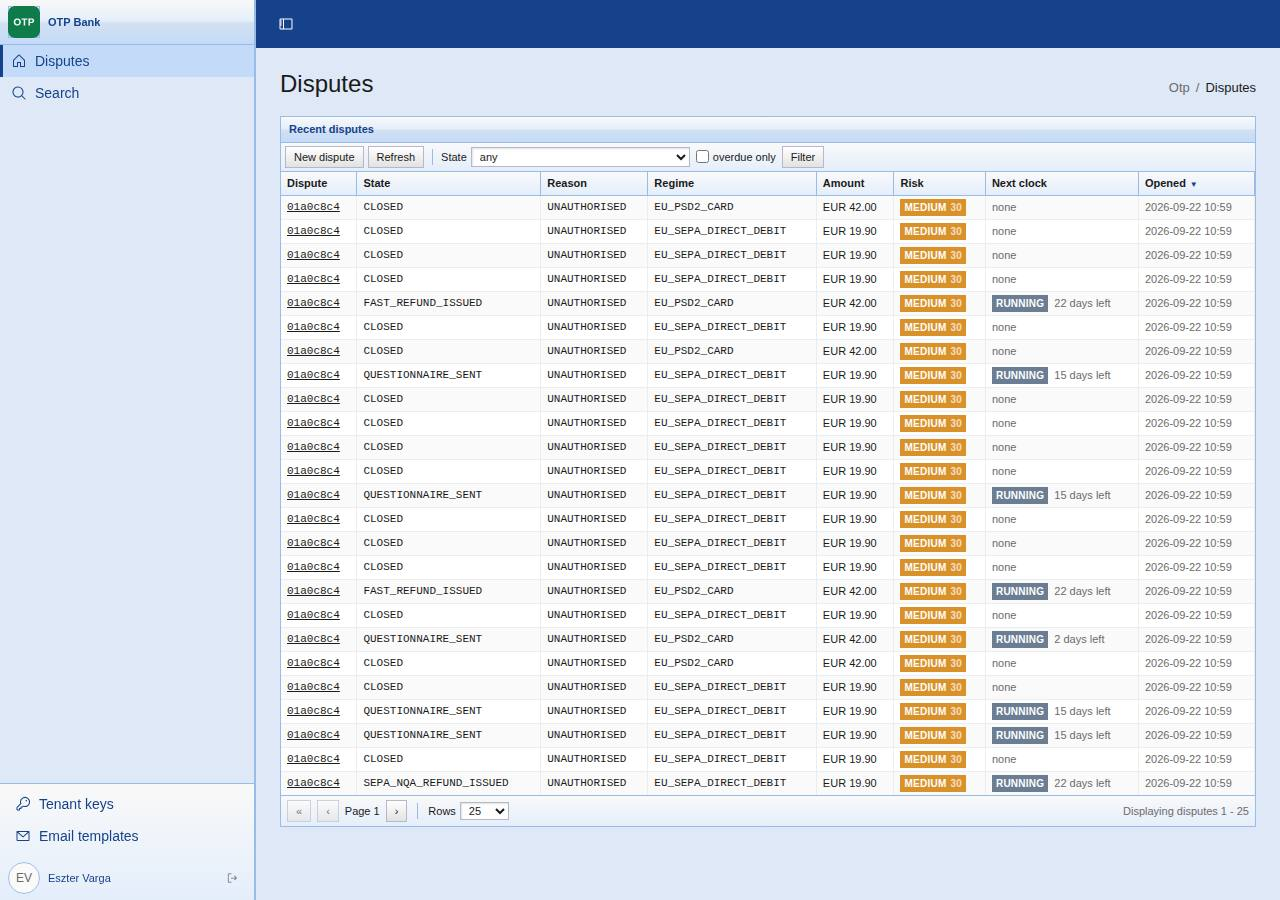
\includegraphics[width=\textwidth]{workbench.jpg}
\caption{The workbench: the organisation and the signed-in analyst on the left, the dispute grid
with its toolbar and pager on the right. Captured against the local stack by
\code{pnpm screenshot}, so it can be retaken after a change rather than going stale.}
\label{fig:workbench}
\end{figure}

\begin{figure}[htbp]
\centering
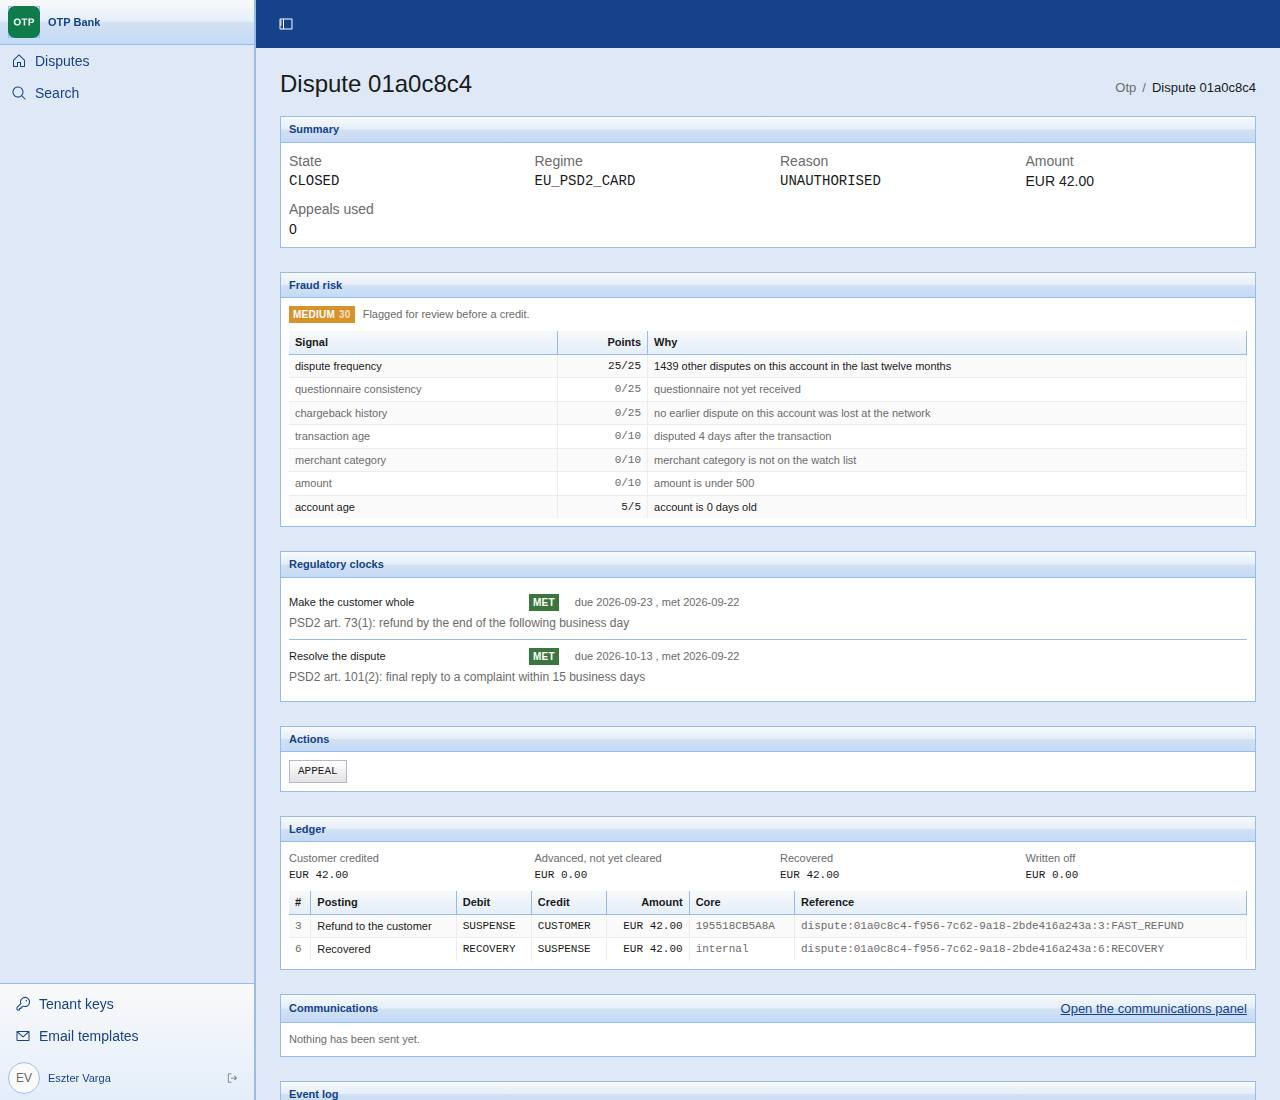
\includegraphics[width=\textwidth]{dispute.jpg}
\caption{One dispute: the summary, the fraud score with the signals that produced it, the
regulatory clocks with their legal basis, and the transitions the state machine allows from the
current state.}
\label{fig:dispute}
\end{figure}

A dispute can also be found directly (figure~\ref{fig:search}): by its identifier, which opens it, or by state and
reason. The grid shows the regime, the amount, the fraud tier with its score and the next running clock with the
time it has left, so an analyst can see which disputes are closest to a legal deadline without opening them. The
list is paginated by the service and ordered by when the dispute opened; the filters are query parameters of the
same list operation the grid uses, so a search result is an ordinary page of the workbench and can be bookmarked.

\begin{figure}[htbp]
\centering
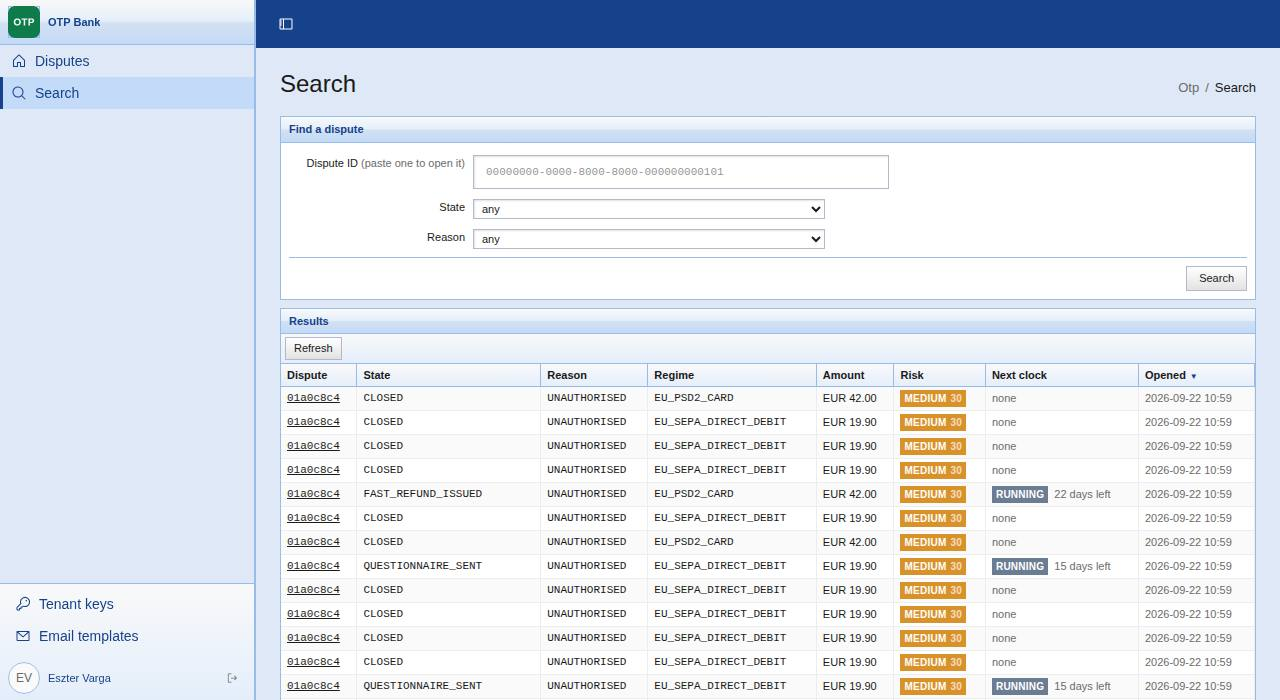
\includegraphics[width=\textwidth]{search.jpg}
\caption{Searching the tenant's disputes by identifier, state or reason. Each row shows its fraud tier and score and
the status of its next clock.}
\label{fig:search}
\end{figure}

\section{Proposals from a typed-decision model}
\label{sec:impl-decisions}

Three places in the workbench turn a person's prose into a value the domain already has a type for: an intake
description becomes one of four reasons, a customer's paragraph becomes typed questionnaire answers, and an
analyst's sentence becomes a set of list filters. A \emph{typed decision model} answers exactly that shape: it
takes a state and questions whose answers are constrained to a closed set, and returns the value with a
probability in one pass, generating no text, so there is nothing to parse.

The model sits behind a port in the application layer beside the banking core of section~\ref{sec:design-core},
for the same reasons: it is someone else's system, it can be slow or down, and the domain must not know which one
it is. It proposes and a person disposes: no transition, clock, posting or letter may depend on it, every use is a
pre-filled field that can be changed, and what is stored is always the value the person left. The port is
optional, so with no model configured these fields are simply empty. A proposal below three quarters
probability is dropped, because a wrong pre-filled answer costs an analyst more attention than an empty one.

Two failures found by driving the real model, rather than a fake, shaped the design more than the benchmark did.
A question offering only the four reasons must answer with one of them: the message ``hello I have a question
about my account'' came back as an unauthorised payment with a confidence comfortably above the gate. The
question now offers an explicit option for text that describes no dispute, and that message yields nothing. Yes
and no questions cannot abstain at all: asked about a message that answers nothing, the model returned a
confident negative to every question on the questionnaire. The batch now carries a gate question asking whether
the message is a customer answering about a disputed payment, and without it nothing is proposed. The remedy for a
forced choice is to give the model somewhere to put its uncertainty rather than to raise the threshold.

When an analyst opens a dispute from a proposed reason, the opened event records what was proposed, how sure the
model was, and whether they kept it, so the acceptance rate is something the running system reports rather than
something the author asserts.

\section{Observability from day one}
\label{sec:impl-observability}

Telemetry was part of the first commit, because a regulated system must be able to show what it did. The engine and the workbench
server use OpenTelemetry \cite{otelspec}, configured only through the standard environment variables; without
them the engine still creates spans but exports nothing, and the workbench server does not start its telemetry at
all. Every request is a span named after its route pattern rather than its address. Every database statement is a
child span named after its query, or after its SQL text when it has no name, with no values recorded
(figure~\ref{fig:trace}). Logs go to standard output and, with the trace's identifiers attached, to the same
backend as the traces, after a redaction step that runs before any destination.

A request from the workbench is one trace across both services: the workbench server opens a span per request and
per server function, and its calls carry the trace context, so the engine's spans join it. Work that happens later
is its own trace, linked to the request that caused it: each queued email stores the trace context of the
transition that owed it, and its delivery links back. No attribute is written with a credential or a customer's
personal data; the redaction step itself is tested on the logs.

Locally the signals land in a Grafana stack that provisions two dashboards, one per service
(figure~\ref{fig:dashboard}), and three alert rules from the repository: more than one percent of responses
failing with a server error, a 99th-percentile latency above one second, and an outbox that is not draining. The
evaluation
of chapter~\ref{ch:evaluation} reads its latency numbers back from these same metrics rather than from a separate
harness. Both figures were captured from the running system with \code{pnpm screenshot:ops} after a load run, so
they can be retaken after a change.

\begin{figure}[htbp]
\centering
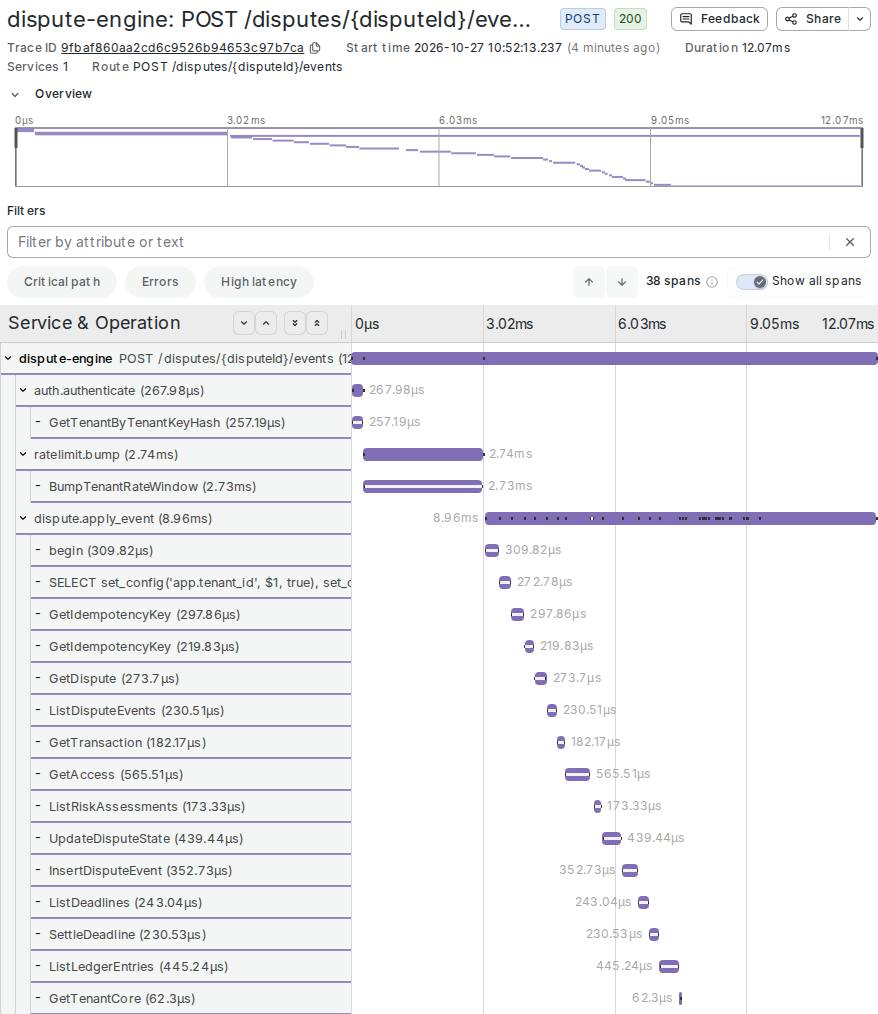
\includegraphics[width=0.85\textwidth]{trace.jpg}
\caption{One transition traced in Tempo: the request, authentication by tenant key, the rate-limit counter, the use
case, and each database statement it ran inside one transaction, 12~ms in total.}
\label{fig:trace}
\end{figure}

\begin{figure}[htbp]
\centering
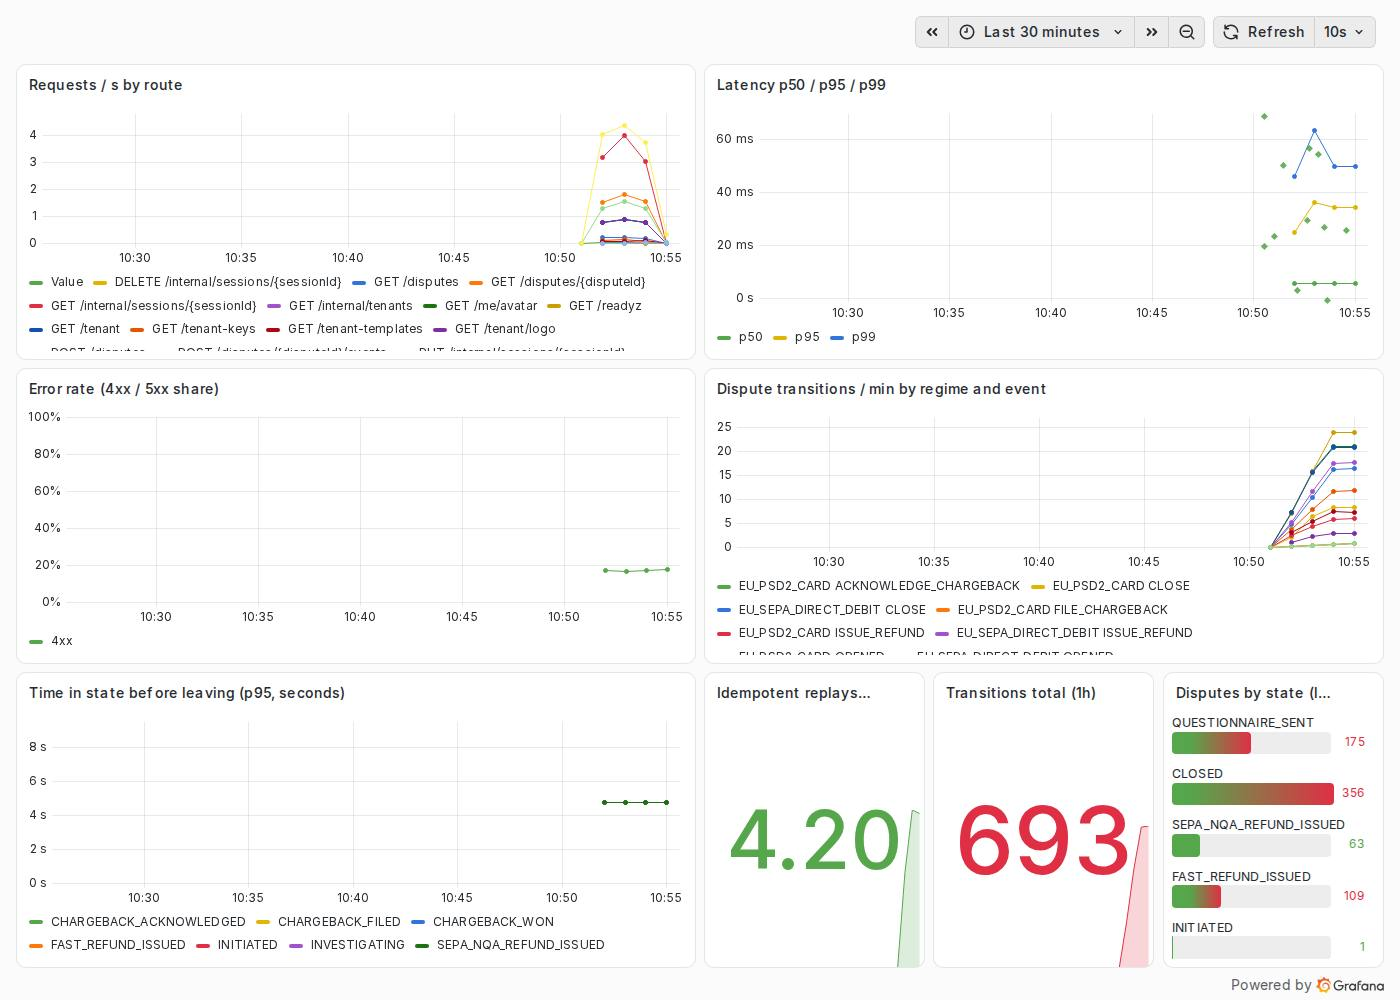
\includegraphics[width=\textwidth]{dashboard.jpg}
\caption{The engine's dashboard during a load run: request rate by route, latency percentiles, the share of client
and server errors (the 4xx line is the run's deliberate refused transitions), transitions by regime and event, time
spent in each state, and disputes by state.}
\label{fig:dashboard}
\end{figure}

\section{Review and release discipline}
\label{sec:impl-ci}

Every change reached the main branch as a pull request, squashed into one commit whose message is the pull
request's title and body; by the time of writing that was 95 merged pull requests and 28 decision records. A
ruleset forbids direct and force pushes, requires signed commits, and requires eight checks to pass on a branch
that is up to date with the main branch, so a change is tested against what it will be merged into.

Continuous integration runs one job per area, with a named step per check, so a failure names its cause
(figure~\ref{fig:ci}). The backend jobs cover formatting, generated code being current, static
analysis, linting, the dependency vulnerability database and the authorization policies, then run the unit and
database-backed suites with the race detector against a real PostgreSQL service. The image job smoke-tests the
backend image the way a deployment would run it: migrations as the owner, then the service as its
least-privileged login, until the readiness endpoint answers. The frontend job generates, type-checks, lints,
tests and builds, and the frontend image is smoke-tested by fetching a page from it. The browser suite reports
but never gates a merge, so that a flaky browser test does not teach everyone to ignore red.

Most of these checks run locally with one command before every push (the vulnerability, policy, race-detector and
integration checks and the image builds are left to continuous integration). Dependabot watches the Go module, the
frontend packages, the workflows and the deployment's container images weekly, and its updates pass the same gate.
Releasing ends at the images, which are built and smoke-tested from any commit on the main branch; the deployment
they would go into is outside the scope of this thesis (section~\ref{sec:req-scope}).

\begin{figure}[htbp]
\centering
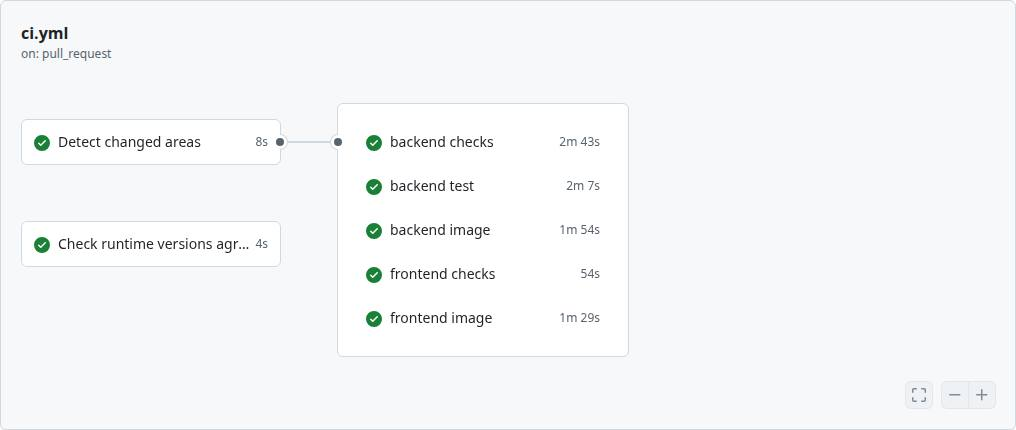
\includegraphics[width=0.8\textwidth]{ci.jpg}
\caption{The continuous-integration jobs of one pull request (the Go toolchain update of
section~\ref{sec:impl-ci}, pull request 107): change detection gates the backend and frontend jobs, and the
version check runs alongside them.}
\label{fig:ci}
\end{figure}

\chapter{Evaluation}
\label{ch:evaluation}

% Budget and sources: docs/thesis/outline.md. Every claim about behaviour points at a test, a figure or a number in data/.


Every number in this chapter comes from run \code{2026-10-19\_1200} in \code{docs/thesis/data}, produced by
\code{make thesis:eval} on a single laptop (Intel i9-14900HX, 32 cores, 30~GB; Go~1.27.1, PostgreSQL~18.6) with
the whole stack running locally. The run executes the test suites, then drives the running service with a paced
load and reads its own metrics back for that window. Section~\ref{sec:eval-decisions} reports a separate, earlier
measurement of the decision model.

\section{Correctness across regimes}
\label{sec:eval-correctness}

The run's suites pass in full: 189 tests across 19 packages. Figure~\ref{fig:eval-coverage} summarises the ones
behind the central claim. For each regime the test explores every state reachable from \emph{initiated}, tries
every event of the transition table in each (the appeal, which sits outside the table, is not part of this walk),
and records which pairs are accepted and which refused. It then fails unless each accepted transition is walked
by at least one named scenario, a dispute taken from \emph{initiated} to \emph{closed} along a readable path such
as ``Regulation~E: chargeback lost without evidence, credit reversed''.

\begin{figure}[htbp]
\centering
\small
\begin{tabular}{lrrrrr}
\toprule
Regime & States & Accepted & Walked & Scenarios & Refused pairs \\
\midrule
SEPA direct debit & 6 & 10 & 10 & 6 & 62 \\
PSD2 card & 11 & 18 & 18 & 8 & 114 \\
Regulation~E & 13 & 20 & 20 & 8 & 136 \\
Regulation~Z & 10 & 16 & 16 & 7 & 104 \\
\midrule
Total & & 64 & 64 & 29 & 416 \\
\bottomrule
\end{tabular}
\caption{Transition coverage per regime in run \code{2026-10-19\_1200} (\code{correctness.json},
\code{TestTransitionCoverage}). States are those reachable from \emph{initiated}; accepted and refused count the
pairs of reachable state and event; walked counts the accepted transitions some named scenario takes.}
\label{fig:eval-coverage}
\end{figure}

Three further tests pin each regime's set of reachable states, require every reachable state to be able to reach
\emph{closed}, and require the events offered in each state to be exactly those accepted, which lets the workbench
show only actions that will succeed. Before the coverage test existed, the named scenarios walked only 28 of the
64 accepted transitions; 23 scenarios were added, and removing the only scenario that walks some transition now
fails the build.

\section{The log, concurrency and retries}
\label{sec:eval-log}

Four tests against a real PostgreSQL database check that the history is trustworthy and retries are safe
(sections~\ref{sec:design-state-machine} and~\ref{sec:design-core}). An update of an event's actor, a delete and
a truncate of the event table are each refused by the database itself. Eight writers applying the same event to
the same dispute at the same instant leave exactly one success; the other seven are refused, as a conflict or as
a transition no longer allowed, and the dispute ends at version two with two events. A request repeated with the
same idempotency key receives the stored response rather than a second dispute, and the same key with a different
body is refused. A forbidden transition writes nothing at all.

Under load, in two minutes, the service opened 479 disputes, applied 958 transitions, replayed one creation in ten
with its original key, and refused one deliberately forbidden event per dispute: 526 creations answered
\code{201} (479 new and 47 replays), 1,437 reads and transitions answered \code{200}, the 479 forbidden events
answered \code{409}, and there were no server errors.

\section{Isolation between tenants and teams}
\label{sec:eval-isolation}

Since isolation must hold even if the application code is wrong (section~\ref{sec:design-tenancy}), it is tested
against the database role the service runs as. Under that role a second tenant cannot read the first tenant's
dispute, apply an event to it, or open a dispute on its transaction, and is answered ``not found'' each time. The
same idempotency key used by two tenants is two separate requests, a connection not bound to a tenant sees no rows,
and inserting a row with another tenant's identifier fails with PostgreSQL's insufficient-privilege error.

Team scope (section~\ref{sec:design-teams}) is tested the same way: an analyst only in another team cannot read,
list or advance a dispute or see its events, and a team lead of another tenant sees nothing, so team scope only
narrows tenant isolation. The authorization policies are checked over generated sets of grants: no set lets an
investigator issue the final credit of a dispute they investigated, reach a dispute outside their teams, or
administer the tenant.

\section{Latency under load}
\label{sec:eval-latency}

The load run measures what a single instance costs per request, not what a deployment could carry. It paced four
lifecycle iterations a second, about twenty requests, for two minutes against one tenant, and read the server's
latency histograms back from Prometheus (figure~\ref{fig:eval-latency}).

\begin{figure}[htbp]
\centering
\small
\begin{tabular}{lrrr}
\toprule
Route & p50 & p95 & p99 \\
\midrule
Read a dispute (\code{GET /disputes/\{id\}}) & 3.3 & 7.2 & 9.5 \\
Apply an event (\code{POST /disputes/\{id\}/events}) & 5.1 & 9.6 & 16.8 \\
Open a dispute (\code{POST /disputes}) & 13.7 & 24.5 & 42.7 \\
\midrule
All requests, as the client saw them & 5.1 & 15.6 & 20.9 \\
\bottomrule
\end{tabular}
\caption{Latency in milliseconds per route, server side, in run \code{2026-10-19\_1200} (\code{load.json}),
at about 20 requests a second for 120 seconds.}
\label{fig:eval-latency}
\end{figure}

An event costs more than a read because one transaction carries the authorization decision, the state machine,
the clocks, the ledger postings, the notices and, where money moves, the call to the simulated core; opening a
dispute also scores it. PostgreSQL was not the bottleneck: its 95th percentile per query was 0.97~ms.

Before authorization existed, the median read took 2.1 milliseconds and the median event 3.0; a policy decision
per operation and team scope in the database raised them to 4.2 and 5.0 (runs \code{2026-09-30\_1050} and
\code{2026-09-30\_1057}), through extra round trips rather than policy evaluation, which costs about 25
microseconds a decision. Against that run, the 99th percentile of opening a dispute rose from 25 to 43
milliseconds with the same code, likely because this run's database-backed suites ran against the same database
just before the load; this has not been isolated.

\section{Are the model's proposals good enough to show?}
\label{sec:eval-decisions}

The feature of section~\ref{sec:impl-decisions} is only defensible if the proposals are usually right, so it was
measured before it was relied on. The labelled set uses the system's own vocabulary: 72 complaints for the four
reasons, 113 answers across 40 replies to the unauthorised questionnaire, and 69 filter fields across 50 queries
over the fifteen states. About a fifth of it is Hungarian (a third of the reasons), since both seeded tenants are
Hungarian banks. An open model on a consumer GPU and a hosted one were run against it (table~\ref{fig:decisions}).

\begin{figure}[htbp]
\centering
\small
\begin{tabular}{lrrrrr}
\toprule
Model & Reason & Questionnaire & Search & ECE & One question \\
\midrule
Open, English checkpoint & 0.597 & 0.469 & 0.812 & 0.401 & 17 ms \\
Open, multilingual & 0.639 & 0.522 & 0.623 & 0.213 & 8 ms \\
Open, typed decisions & 0.639 & 0.611 & 0.696 & 0.595 & 16 ms \\
Hosted & \textbf{0.986} & \textbf{0.973} & \textbf{0.928} & \textbf{0.011} & 574 ms \\
\midrule
Chance & 0.25 & 0.50 & & & \\
\bottomrule
\end{tabular}
\caption{Accuracy on the labelled set (\code{eval/decisions}), expected calibration error on the
reason task, and the latency of one question. The open model runs locally on an RTX~4070; the
hosted one is a network call costing \$0.0000216. Chance is one in four for the reason task and
one in two for the questionnaire.}
\label{fig:decisions}
\end{figure}

The open model is not accurate enough for any of the three uses, and its calibration error means its confidence
cannot decide when to stay quiet. The hosted model's low error is what makes the confidence gate meaningful: its
one wrong reason came back with its probability split between two readings a person would also argue about, and
its three questionnaire mistakes were all one question, which conflated owning the card with carrying it and was
reworded. The set is synthetic, written and labelled by its author, so it measures recovery of a deliberately
encoded intent, an easier task than reading a real customer; the share of proposals analysts keep, which the
running system records, will answer the question properly.

\section{Limitations}
\label{sec:limitations}

The evaluation shows the shape of the system's behaviour, not its capacity: the load ran on one machine shared by
the service, the database, the identity provider and the telemetry stack, from one tenant, with a chosen mix of
synthetic disputes. The correctness results are tests, not proofs, and coverage is over transitions rather than
paths, so a fault that appears only after a particular sequence of steps could be missed. The regimes are modelled
only as far as chapter~\ref{ch:requirements} describes; in particular the banking core is simulated and the card
network's answers are entered by hand, so a real core's behaviour under failure is assumed from its interface
rather than observed. The identity provider's protections, such as multi-factor authentication, are configured
rather than evaluated, and the decision model was measured on a synthetic, self-labelled set
(section~\ref{sec:eval-decisions}).

\chapter{Conclusion and future work}
\label{ch:conclusion}

% Budget and sources: docs/thesis/outline.md. Every claim about behaviour points at a test, a figure or a number in data/.

\section{What the thesis shows}
\label{sec:conclusion-shows}

The thesis set out to show that payment disputes under different regulatory regimes do not need different
software: that one finite state machine, parameterised by the regime, can carry the lifecycle of a PSD2 card
dispute, a SEPA direct-debit claim, a Regulation~E debit-card error and a Regulation~Z billing error, with the
regime deciding which states exist, which deadlines run and which money moves. The engine built to test that claim
carries all four. Its fifteen states are shared, and each regime reaches the part of them its rules describe: six
under SEPA, eleven under PSD2, thirteen under Regulation~E and ten under Regulation~Z. None of the differences is
written as a test of a regime's name; each is a property of the rules, from the kind of money the customer receives
to whether a merchant may contest. The evaluation backs the claim with a test rather than an argument: every one of
the 64 transitions in the four regimes' tables is walked by a named scenario that ends in a closed dispute, and every
pair of state and event a regime forbids is refused (section~\ref{sec:eval-correctness}).

The rest of the work answers the question that follows from the first, which is whether a lifecycle held this way
can bear the weight of a real issuer's process. Deadlines are computed once, in the tenant's own business-day
calendar, and their status is derived on demand, so compliance is a distribution that can be read at any moment
rather than a report assembled afterwards. Money moves once: through a double-entry ledger whose suspense account
is zero whenever a dispute closes, and through a port to the bank's core whose duplicate detection makes a retry
after a timeout safe. Several institutions share one deployment, and the database rather than the code keeps
them apart; the actor on every event is the authenticated caller, and the analyst who investigated a dispute
cannot issue its final credit. These are the properties chapter~\ref{ch:requirements} put above any single feature, and each
is checked by a test, against the real database wherever the database is what enforces it, rather than asserted
(sections~\ref{sec:eval-log} and~\ref{sec:eval-isolation}).

\section{What the decisions cost}
\label{sec:conclusion-costs}

Several decisions bought correctness at a price that the evaluation measured. Taking each authorization decision
inside the request's transaction, on facts already committed, doubled the median latency of a read from about two
to about four milliseconds; the cost is extra round trips to the database rather than the policy engine itself, and
the measurement shows where to recover it without moving the decision (section~\ref{sec:eval-latency}). Calling the
banking core inside the transaction makes the engine as slow as the slowest core it talks to, in exchange for never
recording a refund the core did not make. Keeping PostgreSQL as the only stateful dependency puts every
counter, session and outbox in the same database as the disputes; the measurements show its queries well under a
millisecond at this load, and the reversal is written down as a measurement to wait for rather than a preference.

Other decisions limited what the system claims rather than what it does. Fraud is scored by fixed rules whose
weights are judgement, not fitted to outcomes, and the score may only hold a credit until a person writes down why
it should go out; it never denies a dispute. The typed-decision model is offered to analysts only behind a
confidence gate, and its accuracy was measured on a synthetic set its author labelled. The banking core is a simulator behind a
port, and the card network's answers are entered by hand. Each of these is stated in the text where it applies and collected in
section~\ref{sec:limitations}, so that what the thesis claims and what it measured do not drift apart.

Two parts were marked in the project plan from the outset as the first to cut if time ran short: the fraud-scoring engine and the
analyst-facing workbench. Both were kept, in a form chosen to be defensible rather than impressive. The scoring is
readable and can only slow money down; the workbench never holds a token and shows only the actions the engine would
accept.

\section{Future work}
\label{sec:conclusion-future}

The most direct extensions deepen the lifecycle the thesis already models. The contested rounds of a chargeback
after the merchant's first answer, such as pre-arbitration and arbitration, are folded into one evidence step; they
would become states of their own, gated by the same properties, with deadlines from the card network's rules. The
statutory extensions of deadlines, such as the longer periods Regulation~E allows for new accounts or the holding
reply PSD2 permits in exceptional cases, would become clocks that an event may extend, with the extension recorded
beside the clock it moves. Both are additions to the rules rather than to the machine, which is the test the design
was meant to pass.

The next regulatory step is already visible. The European Union's proposed Payment Services Regulation would extend the issuer's liability to some payments a customer was deceived into authorising, such as
those made to a fraudster impersonating the bank. Under it a dispute may arise from a payment that was authorised, the question becomes whether the bank's own fraud controls
met the expected standard, and the evidence comes from the bank rather than the merchant. That is a new regime in
the sense of this thesis: a row of rules, its clocks and its postings, and a test of whether the gates the four
existing regimes needed are enough for a fifth.

Integration would turn the simulators into adapters. A real core speaks the same instructions and receipts as the
simulated one, so the work is in the adapter and in observing a real core's behaviour when it is slow or silent,
which the port was designed for but has not met. The card network would receive the chargebacks that the engine now only
records, and its answers would become the events that the analyst now enters by hand.

Finally, the two measurements the running system already records would decide two of its open questions. The share
of the decision model's proposals that analysts keep, recorded for the reason proposed when a dispute opens, is the honest
measure of whether the proposals help. And the outcomes of disputes, once there are enough of them, are
the labelled data a learned fraud model would need, against which the fixed rules could be compared rather than
replaced. Both are reasons the engine records what it records: the system was built so that its next decisions can
be taken on evidence, as its first ones were.


\printbibliography[title={Bibliography}]

\appendix
\chapter{Supplementary material}
\label{ch:appendix}

% At most eight to ten pages: API contract excerpt, realm template excerpt, migration listing, raw evaluation tables.

\section{Regulatory clocks per regime}
\label{sec:appendix-clocks}

The deadlines section~\ref{sec:design-clocks} describes, as the engine's rules carry them.

\begin{table}[H]
\centering
\caption{The clocks each regime starts when a dispute opens (\code{domain/regime.go}). Extensions the law
permits for complex cases are not modelled; see section~\ref{sec:limitations}.}
\label{tab:clocks}
\begin{tabular}{llrll}
\tablehead \hd{Regime} & \hd{Clock} & \hd{Count} & \hd{Unit} & \hd{Basis} \\
\rowcolor{tablerow} PSD2 card & refund & 1 & business days & PSD2 art.~73(1) \\
\rowcolor{tablerow}  & resolution & 15 & business days & PSD2 art.~101(2) \\
\rowcolor{white} SEPA Core DD & refund & 10 & business days & PSD2 art.~77(2) \\
\rowcolor{white}  & resolution & 15 & business days & PSD2 art.~101(2) \\
\rowcolor{tablerow} Regulation~E & refund & 10 & business days & 12 CFR 1005.11(c)(2)(i) \\
\rowcolor{tablerow}  & resolution & 45 & calendar days & 12 CFR 1005.11(c)(2) \\
\rowcolor{white} Regulation~Z & acknowledge & 30 & calendar days & 12 CFR 1026.13(c)(1) \\
\rowcolor{white}  & resolution & 90 & calendar days & 12 CFR 1026.13(c)(2) \\
\tableend
\end{tabular}
\end{table}

\clearpage
\section{Ledger postings}
\label{sec:appendix-ledger}

The postings section~\ref{sec:design-ledger} describes, one row per state that causes one.

\begin{table}[H]
\centering
\caption{Postings caused by entering a state (\code{domain/ledger.go}). ``Outstanding'' is the dispute's suspense
balance before the transition; a posting of zero is not written.}
\label{tab:ledger}
\begin{tabular}{L{5.5cm}L{4.1cm}L{2.4cm}L{1.6cm}}
\tablehead \hd{State entered} & \hd{Posting} & \hd{Debit} & \hd{Credit} \\
any credit state & credit (disputed less liability) & suspense & customer \\
\code{PROVISIONAL\_CREDIT\_REVERSED} & reversal (outstanding) & customer & suspense \\
\code{CHARGEBACK\_WON} & recovery (outstanding) & recovery & suspense \\
\code{CHARGEBACK\_LOST}, no provisional credit & write-off (outstanding) & loss & suspense \\
\code{CLOSED}, outstanding & settlement, recovered or written off & recovery or loss & suspense \\
\tableend
\end{tabular}
\end{table}

\clearpage
\section{The dispute page}
\label{sec:appendix-dispute}

\begin{figure}[H]
\centering
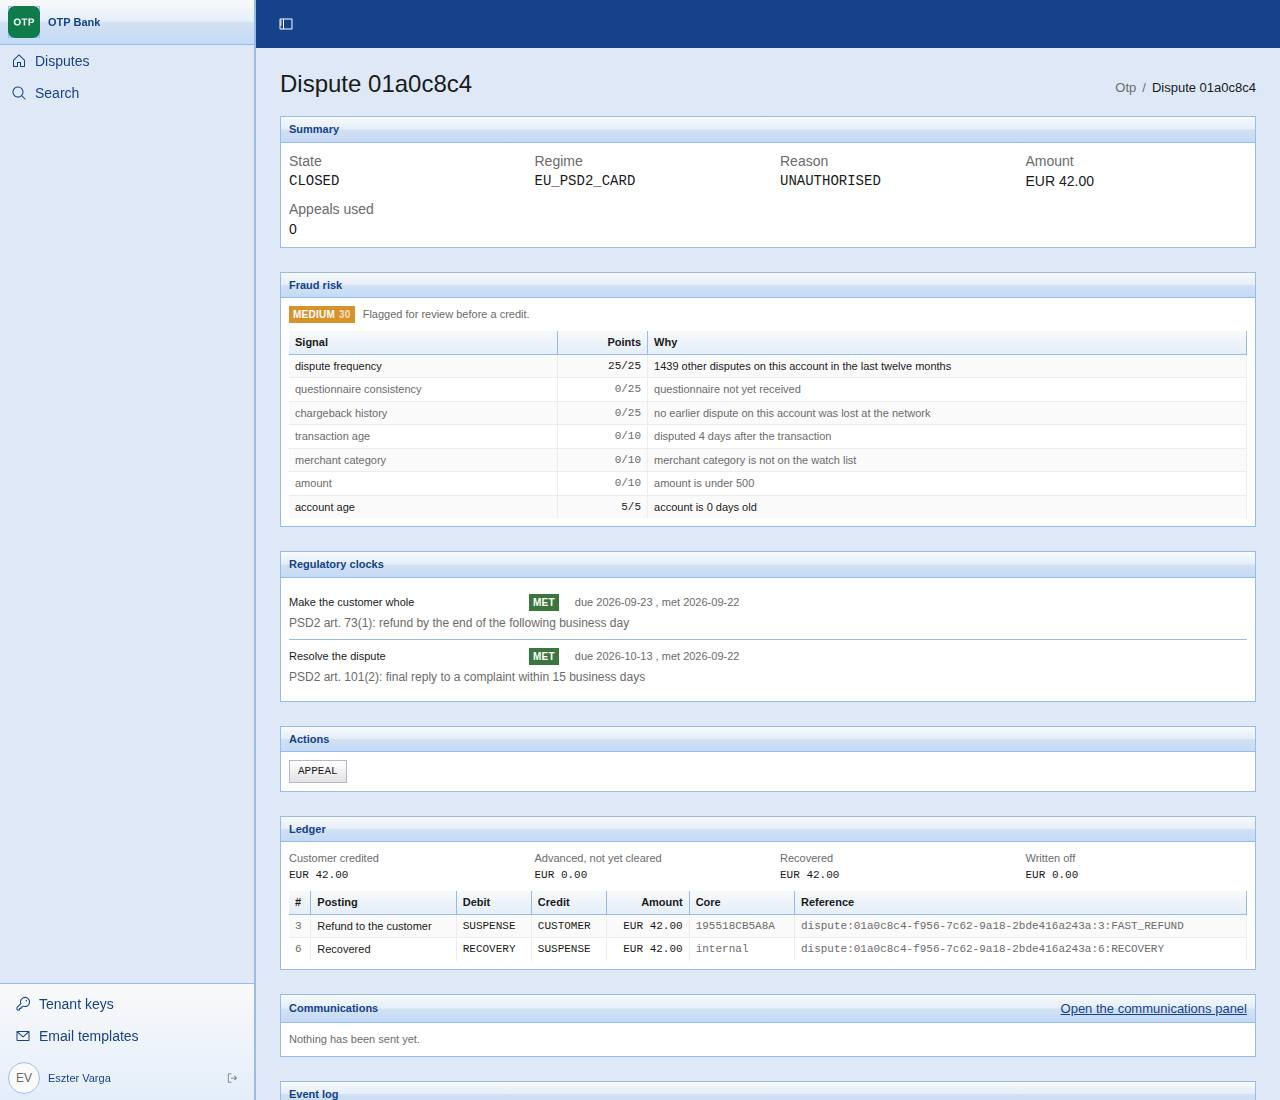
\includegraphics[width=\textwidth]{dispute.jpg}
\caption{One dispute: the summary, the fraud score with the signals that produced it, the
regulatory clocks with their legal basis, and the transitions the state machine allows from the
current state.}
\label{fig:dispute}
\end{figure}

\clearpage
\section{Operating the service}
\label{sec:appendix-operations}

Captured from the running system with \code{pnpm screenshot:ops} after a load run, so they can be retaken after a
change (section~\ref{sec:impl-observability}).

\begin{figure}[H]
\centering
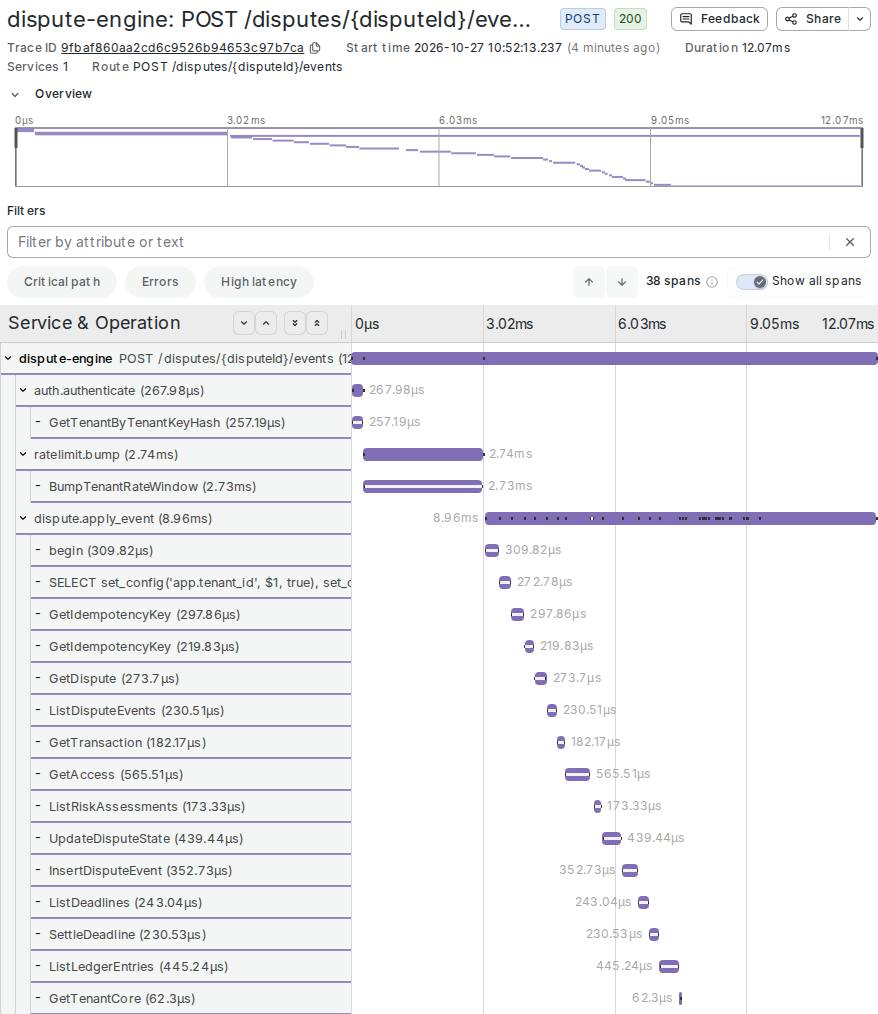
\includegraphics[width=0.85\textwidth]{trace.jpg}
\caption{One transition traced in Tempo: the request, authentication by tenant key, the rate-limit counter, the use
case, and each database statement it ran inside one transaction, 12~ms in total.}
\label{fig:trace}
\end{figure}

\begin{figure}[H]
\centering
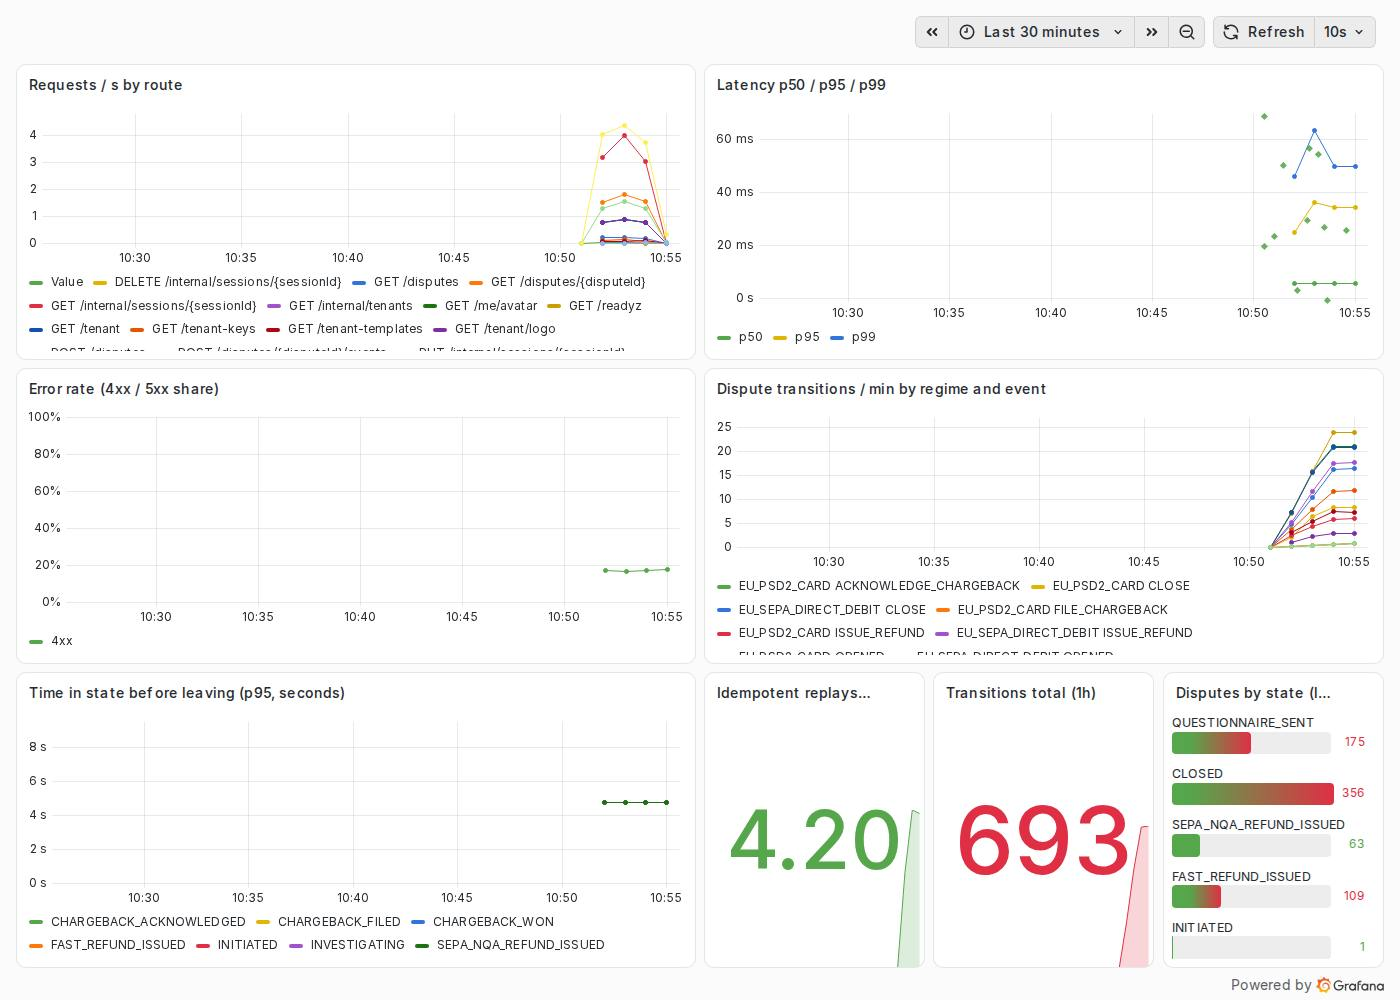
\includegraphics[width=\textwidth]{dashboard.jpg}
\caption{The engine's dashboard during a load run: request rate by route, latency percentiles, the share of client
and server errors (the 4xx line is the run's deliberate refused transitions), transitions by regime and event, time
spent in each state, and disputes by state.}
\label{fig:dashboard}
\end{figure}

\begin{figure}[H]
\centering
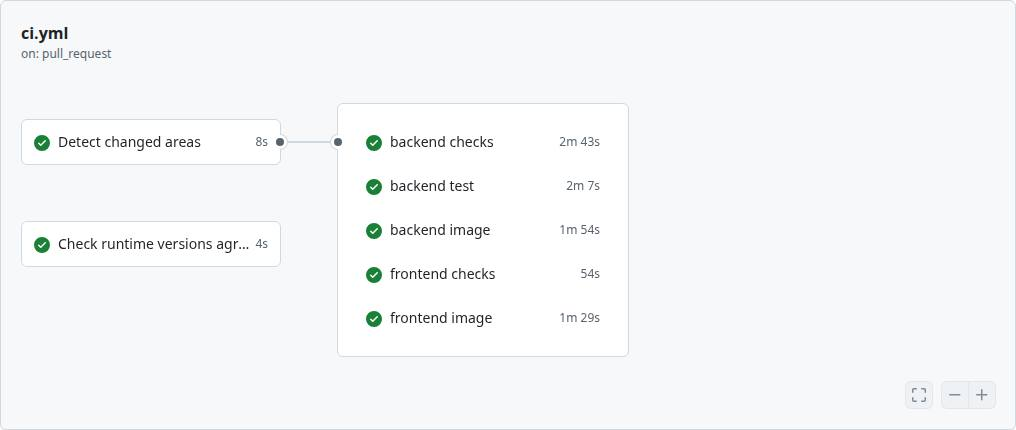
\includegraphics[width=0.8\textwidth]{ci.jpg}
\caption{The continuous-integration jobs of one pull request (the Go toolchain update of
section~\ref{sec:impl-ci}, pull request 107): change detection gates the backend and frontend jobs, and the
version check runs alongside them.}
\label{fig:ci}
\end{figure}

% The faculty's template, "Declaration on the Use of Artificial Intelligence Tools" (inf.unideb.hu/en/information-
% graduating-students-0): its wording kept, its options chosen, its instructional parenthesis removed as it directs.
\clearpage
\phantomsection
\addcontentsline{toc}{chapter}{Declaration on the Use of Artificial Intelligence Tools}
\begin{center}
  {\bfseries Declaration on the Use of Artificial Intelligence Tools\par}
\end{center}
\bigskip

I hereby declare that during the preparation of my thesis I have used the following artificial intelligence-based
tool(s).

\medskip
\noindent\textbf{1. Use of AI tools}

\noindent$\square$ I did not use any artificial intelligence-based tools during the preparation of my thesis.\\
$\boxtimes$ I used artificial intelligence-based tools during the preparation of my thesis as follows

\medskip
\noindent\textbf{Name and version of the AI tool}

\noindent Claude Opus 5.5 (Anthropic), used through Claude Code, Anthropic's command-line coding assistant.

\medskip
\noindent\textbf{Exactly how it was used}

\begin{itemize}\setlength{\itemsep}{0pt}\setlength{\parskip}{0pt}
  \item Programming assistance: drafting code and tests from my specifications, explaining and debugging program
  code, and writing the first versions of configuration and documentation files. All generated code was reviewed,
  run and tested by me, and every change reached the repository as a reviewed pull request.
  \item Design support: proposing alternatives for design decisions, which I then made and recorded as
  architecture decision records.
  \item Text: drafting the chapters of the thesis from my architecture decision records, the repository and the
  committed evaluation runs, followed by shortening, language correction and stylistic refinement. The scope, the
  choice of regimes, the decisions argued for and the structure of each chapter are mine.
  \item Figures and tables: preparing the scripts that generate diagrams from the code and capture screenshots of
  the running system. Every number in the evaluation comes from a committed measurement run, not from the tool.
  \item Verification: checking the claims of the text against the code, the tests and the measurements, and the
  legal citations against their sources, which I then confirmed myself.
\end{itemize}

\medskip
\noindent\textbf{2. Declaration of independent work}

I declare that I take full responsibility for the professional content of my thesis. I acknowledge that the use
of artificial intelligence-based tools does not replace independent work; therefore, I have verified all
statements, results, interpretations, conclusions, and references included in the thesis.

I further declare that:
\begin{itemize}\setlength{\itemsep}{0pt}\setlength{\parskip}{0pt}
  \item the final content of the thesis was compiled by me,
  \item any AI-generated or modified content has been reviewed, verified, and corrected where necessary,
  \item the original results, interpretations, and conclusions presented in the thesis are my responsibility,
  \item the use of AI tools has been truthfully and fully disclosed in this declaration.
\end{itemize}

\chapter*{Acknowledgements}
\addcontentsline{toc}{chapter}{Acknowledgements}

% Written last.


\end{document}
